% Options for packages loaded elsewhere
\PassOptionsToPackage{unicode}{hyperref}
\PassOptionsToPackage{hyphens}{url}
%
\documentclass[
]{book}
\usepackage{amsmath,amssymb}
\usepackage{lmodern}
\usepackage{ifxetex,ifluatex}
\ifnum 0\ifxetex 1\fi\ifluatex 1\fi=0 % if pdftex
  \usepackage[T1]{fontenc}
  \usepackage[utf8]{inputenc}
  \usepackage{textcomp} % provide euro and other symbols
\else % if luatex or xetex
  \usepackage{unicode-math}
  \defaultfontfeatures{Scale=MatchLowercase}
  \defaultfontfeatures[\rmfamily]{Ligatures=TeX,Scale=1}
\fi
% Use upquote if available, for straight quotes in verbatim environments
\IfFileExists{upquote.sty}{\usepackage{upquote}}{}
\IfFileExists{microtype.sty}{% use microtype if available
  \usepackage[]{microtype}
  \UseMicrotypeSet[protrusion]{basicmath} % disable protrusion for tt fonts
}{}
\makeatletter
\@ifundefined{KOMAClassName}{% if non-KOMA class
  \IfFileExists{parskip.sty}{%
    \usepackage{parskip}
  }{% else
    \setlength{\parindent}{0pt}
    \setlength{\parskip}{6pt plus 2pt minus 1pt}}
}{% if KOMA class
  \KOMAoptions{parskip=half}}
\makeatother
\usepackage{xcolor}
\IfFileExists{xurl.sty}{\usepackage{xurl}}{} % add URL line breaks if available
\IfFileExists{bookmark.sty}{\usepackage{bookmark}}{\usepackage{hyperref}}
\hypersetup{
  pdftitle={Climate Change},
  pdfauthor={Dyrehaugen Web Notebook},
  hidelinks,
  pdfcreator={LaTeX via pandoc}}
\urlstyle{same} % disable monospaced font for URLs
\usepackage{longtable,booktabs,array}
\usepackage{calc} % for calculating minipage widths
% Correct order of tables after \paragraph or \subparagraph
\usepackage{etoolbox}
\makeatletter
\patchcmd\longtable{\par}{\if@noskipsec\mbox{}\fi\par}{}{}
\makeatother
% Allow footnotes in longtable head/foot
\IfFileExists{footnotehyper.sty}{\usepackage{footnotehyper}}{\usepackage{footnote}}
\makesavenoteenv{longtable}
\usepackage{graphicx}
\makeatletter
\def\maxwidth{\ifdim\Gin@nat@width>\linewidth\linewidth\else\Gin@nat@width\fi}
\def\maxheight{\ifdim\Gin@nat@height>\textheight\textheight\else\Gin@nat@height\fi}
\makeatother
% Scale images if necessary, so that they will not overflow the page
% margins by default, and it is still possible to overwrite the defaults
% using explicit options in \includegraphics[width, height, ...]{}
\setkeys{Gin}{width=\maxwidth,height=\maxheight,keepaspectratio}
% Set default figure placement to htbp
\makeatletter
\def\fps@figure{htbp}
\makeatother
\setlength{\emergencystretch}{3em} % prevent overfull lines
\providecommand{\tightlist}{%
  \setlength{\itemsep}{0pt}\setlength{\parskip}{0pt}}
\setcounter{secnumdepth}{5}
\usepackage{booktabs}
\usepackage{amsthm}
\makeatletter
\def\thm@space@setup{%
  \thm@preskip=8pt plus 2pt minus 4pt
  \thm@postskip=\thm@preskip
}
\makeatother

\renewcommand\chaptername{}
\ifluatex
  \usepackage{selnolig}  % disable illegal ligatures
\fi
\usepackage[]{natbib}
\bibliographystyle{apalike}

\title{Climate Change}
\author{Dyrehaugen Web Notebook}
\date{2021-02-01}

\begin{document}
\maketitle

{
\setcounter{tocdepth}{1}
\tableofcontents
}
\hypertarget{climate-change}{%
\chapter{Climate Change}\label{climate-change}}

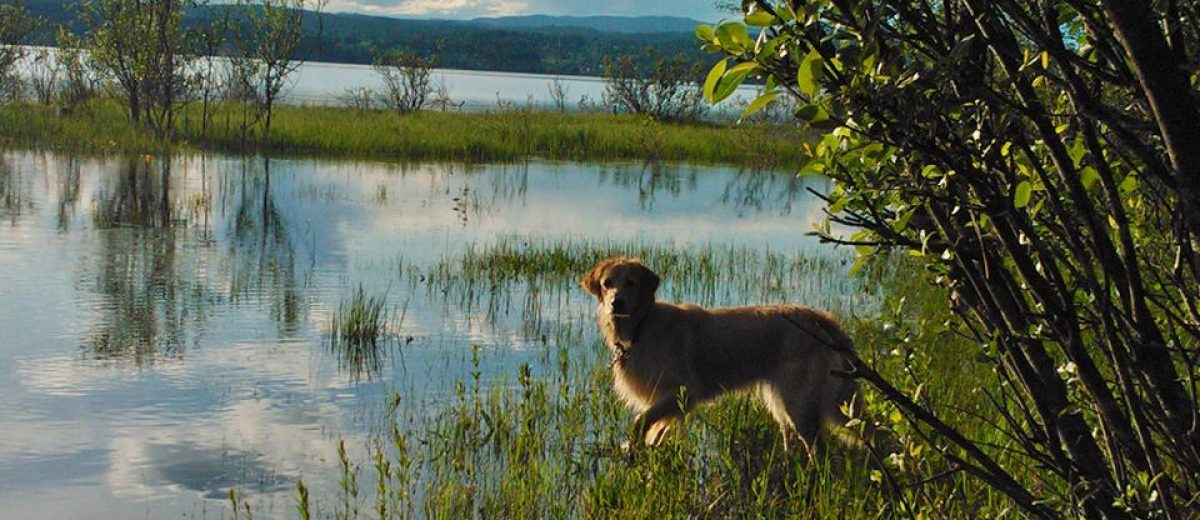
\includegraphics{fig/zelda.jpg}

\hypertarget{part-climate-models}{%
\part{Climate Models}\label{part-climate-models}}

\hypertarget{climate-models}{%
\chapter{Climate Models}\label{climate-models}}

Overview text on selected Climate Models

\hypertarget{dice-climate-model}{%
\section{DICE Climate Model}\label{dice-climate-model}}

Independent of the
normative assumptions of inequality aversion and time preferences,
the Paris agreement constitutes the economically optimal policy pathway
for the century.
Authors claim they show this by incorporating a
damage-cost curve reproducing
the observed relation between temperature
and economic growth into the integrated assessment model DICE.

\href{https://www.nature.com/articles/s41467-019-13961-1}{Glanemann (2021) DICE Paris CBA}
\href{pdf/Glanemann_2021_DICE_Paris_CBA.pdf}{(pdf)}

\hypertarget{ez-climate-model}{%
\section{EZ-Climate Model}\label{ez-climate-model}}

Some text on EZClimate

\hypertarget{fair-climate-model}{%
\section{FAIR Climate Model}\label{fair-climate-model}}

The FAIR model satisfies all
criteria set by the NAS for use in an SCC calculation. 22 Importantly, this model
generates projections of future warming that are consistent with comprehensive, state-
of-the-art models and it can be used to accurately characterize current best
understanding of the uncertainty regarding the impact that an additional ton of CO 2
has on global mean surface temperature (GMST). Finally, FAIR is easily implemented
and transparently documented, 23 and is already being used in updates of the SCC. 24

A key limitation of FAIR and other simple climate models is that they do not represent
the change in global mean sea level rise (GMSL) due to a marginal change in emissions.

\href{Greenstone_2021_Updating_SCC.pdf}{Carleton Greenstone (2021) Updating SCC (pdf)}

\href{https://fair.readthedocs.io/en/latest/}{FAIR}

\hypertarget{monash-climate-model}{%
\section{Monash Climate Model}\label{monash-climate-model}}

Some text on Monash Model

\hypertarget{noresm}{%
\section{NorESM}\label{noresm}}

\textbf{Norwegian Earth System Model}

\emph{About}

A climate model solves mathematically formulated natural laws on a three-dimensional grid. The climate model divides the soil system into components (atmosphere, sea, sea ice, land with vegetation, etc.) that interact through transmission of energy, motion and moisture. When the climate model also includes advanced interactive atmosphere chemistry and biogeochemical cycles (such as the carbon cycle), it is called an earth system model.

The Norwegian Earth System Model NorESM has been developed since 2007 and has been an important tool for Norwegian climate researchers in the study of the past, present and future climate. NorESM has also contributed to climate simulation that has been used in research assessed in the IPCC's fifth main report.

\emph{INES}

The project Infrastructure for Norwegian Earth System Modeling (INES) will support the further development of NorESM and help Norwegian scientists also gain access to a cutting-edge earth system model in the years to come. Technical support will be provided for the use of a more refined grid, the ability to respond to climate change up to 10 years in advance, the inclusion of new processes at high latitudes and the ability of long-term projection of sea level.
Climate simulations with NorESM are made on some of the most powerful supercomputers in Norway, and INES will help these exotic computers to be exploited in the best possible way and that the large data sets produced are efficiently stored and used. The project will ensure that researchers can efficiently use the model tool, analyze results and make the results available.

\href{https://www.noresm.org/}{NorESM}

\href{https://gmd.copernicus.org/articles/6/687/2013/}{Bentsen (2013) NorESM - Part 1}
\href{pdf/Bentsen_2013_NorESM_1.pdf}{(pdf)}

\href{https://gmd.copernicus.org/articles/6/389/2013/}{Iversen (2013) NorESM - Part 2}
\href{pdf/Iversen_2013_NorESM_2.pdf}{(pdf)}

\hypertarget{goal-index}{%
\section{Goal Index}\label{goal-index}}

In economic modelling choice of goal index (utility) function matters.
Daniel 2018\footnote{See Links to references} presents this figure:

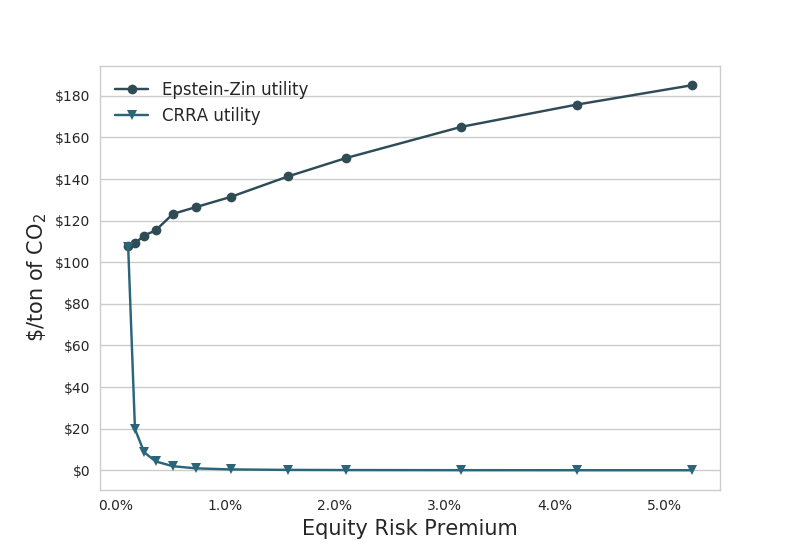
\includegraphics{fig/fig_EZvsCRRA_daniel2018fig1.png}

Fig. Optimal CO2-prices with increasing risk aversion for EZ vs CRRA utility specification. (From Daniel 2018)

As one of the co-authors explain: `We where not able to get the Social
Cost of Carbon (SCC) under \$120'.
That is for `reasonable risk aversion', using EZ-utilities.
The `standard' specification - with CRRA - utilities ends up with SCC
of \$20 or below.

\[V_1 = A [\tilde{C\_t}, \mu_t(V\_{t+1})]\]

Specification of the Goal Index function may seem a trivial technical issue -
no so!
There exists a broad professional litterature and profound discussions on
this matter -
which might de difficult to dis-entangle.

Let us begin with Frank Ramsey's growth model from 1928, commonly known
as the Ramsey-Cass-Koopmans model.

\(F(K,L)\) is an aggregate production function with factors \(K\) (Capital) and
\(L\) (Labour).

\hypertarget{model-drift}{%
\section{Model Drift}\label{model-drift}}

\emph{Abstract Sausen}

A method is proposed for removing the
drift of coupled atmosphere-ocean models, which
in the past has often hindered the application of
coupled models in climate response and sensitivity experiments.
The ocean-atmosphere flux fields
exhibit inconsistencies when evaluated separately
for the individual sub-systems in independent,
uncoupled mode equilibrium climate computations.
In order to balance these inconsistencies a
constant ocean-atmosphere flux correction field is
introduced in the boundary conditions coupling
the two sub-systems together. The method ensures
that the coupled model operates at the reference
climate state for which the individual model subsystems
were designed without affecting the dynamical response of the coupled system in climate
variability experiments. The method is illustrated
for a simple two component box model and an
ocean general circulation model coupled to a two
layer diagnostic atmospheric model.

\emph{Memo Barthel}

The coupling of different climate sub-systems poses a number of technical
problems. An obvious problem arising from the
different time scales is the synchronization or
matching of the numerical integration of subsys-
tems characterized by widely differing time steps.
A more subtle problem is

\emph{Model Drift}
When two general circulation models of the
atmosphere and ocean are coupled together in a
single model, it is generally found that the cou-
pled system gradually drifts into a new climate
equilibrium state which is far removed from the
observed climate. The coupled model climate
equilibrium may be so unrealistic (for example,
with respect to sea ice extent, or the oceanic equa-
torial current system) that climate response or
sensitivity experiments relative to this state be-
come meaningless. This occurs regularly even
when the individual models have been carefully
tested in detailed numerical experiments in the
decoupled mode and have been shown to yield
satisfactory simulations of the climate of the sepa-
rate ocean or atmosphere sub-systems.
The drift of the coupled model is clearly a sign
that something is amiss with the models. Howev-
er, we suggest that it is not necessary to wait with
climate response and sensitivity experiments with
coupled models unit all causes of model drift
have been properly identified and removed.
Model drift is, in fact, an extremely sensitive indi-
cator of model imperfections. The fact that the
equilibrium climate into which a coupled model
drifts is unacceptably far removed from the real
climate does not necessarily imply that the model
dynamics are too unrealistic for the model to be
applied for climate response and sensitivity ex-
periments. One should therefore devise methods
for separating the drift problem from the basically
independent problem of determining the change
of the simulated climate induced by a change in
boundary conditions a n d / o r external forcing (cli-
mate response), and from the question of the ef-
fect of changes in the physical or numerical for-
mulation of the model (model sensitivity).

\emph{Flux Correction}
The separation of the mean climate
simulation from the climate response or sensitiv-
ity problem can be achieved for coupled models
rather simply by an alternative technique, the flux
correction method.
The errors that result in a drift of the coupled
model are compensated in this method by con-
stant correction terms in the flux expressions by
which the separate sub-system models are cou-
pled together. The correction terms have no in-
fluence on the dynamics of the system in climate
response or sensitivity experiments, but ensure
that the ``working point'' of the model lies close to
the climate state for which the individual models
were originally tuned.
The basic principle of the flux correction method
is to couple the atmosphere and the ocean in such
a manner that in the unperturbed case each sub-
system simulates its own mean climate in the
same manner as in the uncoupled mode, but re-
sponds fully interactively to the other sub-system
in climate response or sensitivity experiments.

\href{pdf/Barthel_1988_Coupled_ocean_atmosphere_models_with_flux_corection.pdf}{Sausen (1988) Coupled Ocean-Atmosphere Model Drift Flux Correction (pdf)}

\hypertarget{part-measurements}{%
\part{Measurements}\label{part-measurements}}

\hypertarget{attribution}{%
\chapter{Attribution}\label{attribution}}

For too long, weather's randomness has kept events such as these from being blamed squarely on climate change. Reporters in the late 1990s and early 2000s would ask climate scientists about climate change's role in a weather-related disaster. All we could say was that we'd expect to see more of these events. Now, we can specify increased chances for specific events. This extends to forecasts: we can identify the places that are more likely to see wildfires, mudslides and fish die-offs. Such calculations dent both climate denial and a false sense of security. They take away the argument that `extreme weather happens anyway, so we don't need to worry about it'. Extreme weather happens --- and these metrics pinpoint what is becoming more likely, by how much and why.

\href{https://www.nature.com/articles/d41586-021-00185-x}{Betts (2021) Nature}

\href{https://www.ametsoc.org/ams/index.cfm/publications/bulletin-of-the-american-meteorological-society-bams/explaining-extreme-events-from-a-climate-perspective/}{Ametsoc (2021) Explaining Extreme Weather}
\href{pdf/Ametsoc_2021_Explaining_Extreme_2019.pdf}{(pdf)}

\hypertarget{carbon-budget}{%
\chapter{Carbon Budget}\label{carbon-budget}}

\begin{quote}
The temperature response for a 1.5°C scenario has a huge uncertainty \& this propagates to the uncertainty in the carbon budget.
To say ``the remaining carbon budget for 1.5°C is 440 GtCO₂'' {[}add favorite number{]} is highly misleading
Taking a narrow 67--33\% range, the value is 230--670 GtCO₂, but full range (left) could be −1000 - 2000 GtCO₂\ldots{} (yes, could be negative or huge)
(Glen Peters)
\end{quote}

\emph{Memo Matthews:}

The remaining carbon budget quantifies the future CO 2 emissions to limit global warming
below a desired level. Carbon budgets are subject to uncertainty in the Transient Climate
Response to Cumulative CO 2 Emissions (TCRE), as well as to non-CO 2 climate influences.
We estimate a median TCRE of 0.44 °C and 5--95\% range of 0.32--0.62 °C per 1000 GtCO 2
emitted. Considering only geophysical uncertainties, our median estimate of the 1.5 °C
remaining carbon budget is 440 GtCO 2 from 2020 onwards, with a range of 230--670
GtCO 2 , (for a 67--33\% chance of not exceeding the target). Additional socioeconomic
uncertainty related to human decisions regarding future non-CO 2 emissions scenarios can
further shift the median 1.5 °C remaining carbon budget by ±170 GtCO 2 .

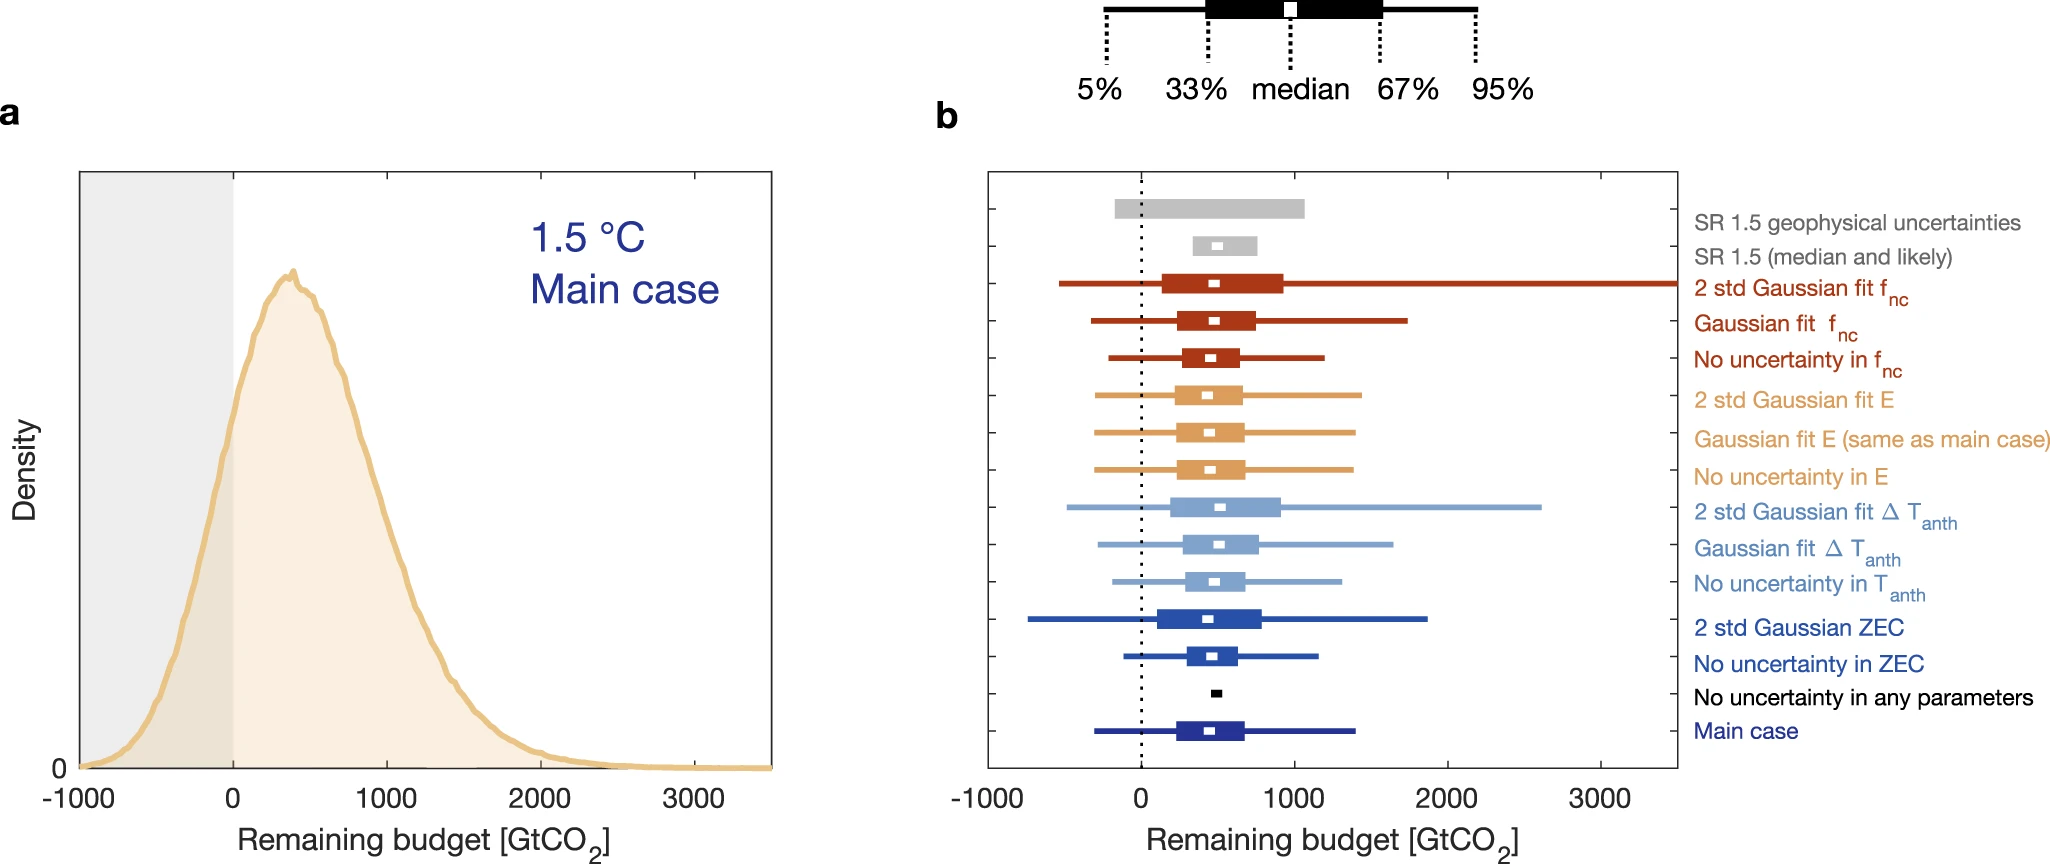
\includegraphics{fig/carbon_budget.png}

Remaining carbon budgets (RCBs) represent the future
cumulative CO 2 emissions that would be consistent with
keeping global warming to a specified level.
Despite being conceptually simple, RCBs have been
defined and estimated in various ways and with many different
underlying assumptions, resulting in a wide range of
``best estimates'' across different studies 2 . Moreover, most of these
estimates of remaining budgets account for only a subset of the
relevant uncertain processes and often omit the contribution of
key uncertain processes (such as permafrost thaw or future
scenario uncertainty, among others)

Median TCRE estimate is 0.44 °C per 1000 GtCO2 , with a 5--95\%
range of 0.32--0.62 °C per 1000 GtCO2

A stronger constraint on the left-hand side of the distribution (low
TCRE values, with sharply increasing probability above 0.25 °C/
1000 GtCO 2 ), while the right-hand side of this distribution has a
wider tail. This right-skewed distribution shape of our
observationally-constrained TCRE estimate is physically related
to the possibility of a large negative aerosol forcing

Median RCB for 1.5 °C is 440 GtCO2 from 2020
onwards, representing a 50\% chance of stabilising warming at or
below 1.5 °C.
The corresponding budget for a 67\% chance of remaining below the target is
230 GtCO2 from the year 2020 onwards.

\href{https://www.nature.com/articles/s43247-020-00064-9}{Matthews(2021) Carbon Budget Uncertainties}
\href{pdf/Matthews_2021_Carbon_Budget_Uncertainties.pdf}{(pdf)}

\hypertarget{climate-feedbacks}{%
\chapter{Climate Feedbacks}\label{climate-feedbacks}}

\emph{Abstract Heinze}
Earth system models (ESMs) are key tools for providing climate projections under different sce-
narios of human-induced forcing. ESMs include a large number of additional processes and feedbacks such as
biogeochemical cycles that traditional physical climate models do not consider. Yet, some processes such as
cloud dynamics and ecosystem functional response still have fairly high uncertainties. In this article, we present
an overview of climate feedbacks for Earth system components currently included in state-of-the-art ESMs and
discuss the challenges to evaluate and quantify them. Uncertainties in feedback quantification arise from the in-
terdependencies of biogeochemical matter fluxes and physical properties, the spatial and temporal heterogeneity
of processes, and the lack of long-term continuous observational data to constrain them. We present an outlook
for promising approaches that can help to quantify and to constrain the large number of feedbacks in ESMs in
the future. The target group for this article includes generalists with a background in natural sciences and an
interest in climate change as well as experts working in interdisciplinary climate research (researchers, lecturers,
and students). This study updates and significantly expands upon the last comprehensive overview of climate
feedbacks in ESMs, which was produced 15 years ago (NRC, 2003).

\href{https://www.researchgate.net/publication/334387499_ESD_Reviews_Climate_feedbacks_in_the_Earth_system_and_prospects_for_their_evaluation}{Heinze (2019) Climate Feedbacks}
\href{pdf/Heinze_2019_Climate_Feedbacks.pdf}{(pdf)}

\hypertarget{climate-sensitivity}{%
\chapter{Climate Sensitivity}\label{climate-sensitivity}}

\emph{ECS}

Climate sensitivity is defined as the equilibrium change in global and annual mean
surface air temperature, \(\Delta T\), due to an increment in
downward radiative flux, \(\Delta R_{f}\) ,
that would result from sustained doubling of atmospheric \(CO_2\) over its
preindustrial value (2 x \(CO_2\) ).

Studies based, on observations, energy balance models, temperature reconstructions,
and global climate models (GCMs) have found that the probability
density distribution of \(\Delta T\) is peaked in the range
2.0°C ≤ \(\Delta T\) ≤ 4.5°C, with a long tail of small but
finite probabilities of very large temperature increases.

An important parameter in climate science is
the equilibrium or long-run response in the global mean surface temperature
to a doubling of atmospheric carbon dioxide.

In the climate science community, this is called
the equilibrium climate sensitivity ECS.
With reference to climate models, this is calculated as
the increase in average surface temperature with a doubled CO2 concentration
relative to a path with the pre-industrial CO2 concentration.
This parameter also plays a key role in the geophysical components
in the IAMs.

Given the importance of the ECS in climate science,
there is an extensive literature estimating probability density functions.
These pdfs are generally based on climate models, the instrumental
records over the last century or so, paleoclimatic data such
as estimated temperature and radiative forcings over ice-age intervals,
and the results of volcanic eruptions.
Much of the literature estimates a probability density function
using a single line of evidence,
but a few papers synthesize different studies or different kinds of evidence.

The IPCC Fifth Assessment report (AR5) reviewed the literature
quantifying uncertainty in the ECS and highlighted
five recent papers using multiple lines of evidence (IPCC, 2014).
Each paper used a Bayesian approach to update a prior distribution
based on previous evidence
(the prior evidence usually drawn from instrumental records or a climate model)
to calculate the posterior probability density function.

\href{https://globalchange.mit.edu/publication/16235}{Gilligham (2015) Modelling Uncertainty}
\href{pdf/Gillingham_2015_Modelling_Uncertainty.pdf}{(pdf)}

\hypertarget{roe-and-baker-distribution}{%
\section{Roe and Baker Distribution}\label{roe-and-baker-distribution}}

\emph{Abstract}

Uncertainties in projections of future climate change have not lessened substantially in past
decades. Both models and observations yield broad probability distributions for long-term
increases in global mean temperature expected from the doubling of atmospheric carbon dioxide,
with small but finite probabilities of very large increases. We show that the shape of these
probability distributions is an inevitable and general consequence of the nature of the climate
system, and we derive a simple analytic form for the shape that fits recent published distributions
very well. We show that the breadth of the distribution and, in particular, the probability of
large temperature increases are relatively insensitive to decreases in uncertainties associated with
the underlying climate processes.

\emph{Memo Roe and Baker}

What determines the distribution shape of ECS and in particular, the high \(\Delta T\) tail?
To what extent we can decrease the distribution width?

Climate consists of a set of highly coupled, tightly interacting physical processes.
Understanding these physical processes is a massive
task that will always be subject to uncertainty.
How do the uncertainties in the physical processes translate into an uncertainty in climate
sensitivity?

Explanations for the range of
predictions of DT, summarized in (14), have
focused on
(i) uncertainties in our understanding of the individual physical processes
(in particular, those associated with clouds),
(ii) complex interactions among the individual processes, and
(iii) the chaotic, turbulent nature of the climate system, which may give rise to
thresholds, bifurcations, and other discontinuities, and which
remains poorly understood on a theoretical level.
We show here that the explanation is far more fundamental than any of these.

We use the framework of feedback analysis to examine the relationship between the
uncertainties in the individual physical processes and the ensuing shape of
the probability distribution of \(\Delta T\).
Because we are considering an equilibrium temperature rise, we consider only
time-independent processes.

\href{https://www.semanticscholar.org/paper/Why-Is-Climate-Sensitivity-So-Unpredictable-Roe-Baker/9a0c81f6887db897000dbce576b139a486f62c77}{Roe and Baker (2007) Climate Sensitivity}
\href{pdf/Roe_Baker_2007_Climate_Sensitivity.pdf}{(pdf)}

\emph{Memo Hannart}

RB addressed these questions using rather simple
theoretical considerations and reached the conclusion that
reducing uncertainties on climate feedbacks and underlying
climate processes will not yield a large reduction in the
envelope of climate sensitivity. In this letter, we revisit the
premises of this conclusion. We show that it results from a
mathematical artifact caused by a peculiar definition of
uncertainty used by these authors.

Reducing inter-model spread on
feedbacks does in fact induce a reduction of uncertainty on
climate sensitivity, almost proportionally.
Therefore, following Roe and Baker assumptions, climate sensitivity is actually
not so unpredictable.

The main originality of RB07 approach consists in analyzing
explicitly the way uncertainties on \(f\), due to a limited
understanding of their underlying physical processes, prop-
agates into uncertainties on \(\Delta T\): assuming \(f\) is a random
variable with mean \(f\) and standard deviation \(\sigma_f\) , RB07 uses
this simple probabilistic model to highlight several fundamental
properties of uncertainty propagation from feedbacks
to climate sensitivity. The most prominent conclusion of this
analysis is that reducing uncertainties on \(f\) does not yield a
large reduction in the uncertainty of \(\Delta T\), and thus that
improvements in the understanding of physical processes
will not yield large reductions in the envelope of future
climate projections.
We show that this conclusion is a mathematical artifact
with no connection whatsoever to climate.

RB07 uses the feedback analysis framework.
Denoting \(\Delta T_0\) the Planck temperature response to the radiative
perturbation and \(f\) the feedback gain (RB07 refers to it as
feedback factor), they obtain:

\[\Delta T = \frac{\Delta T_0}{1 - f}\]

RB07 then assumes uncertainty on Planck response to be
negligible so that the entire spread on \(\Delta T\) results from the
uncertainty on the global feedback gain \(f\). To model this
uncertainty, RB07 assumes that \(f\) follows a Gaussian
distribution with mean \(\overline{f}\) , standard deviation \(\sigma_f\) and implicit
truncation for \(f\) \textgreater{} 1.
Then, they derive an exact expression of the distribution of \(\Delta T\).
This simple probabilistic climatic model is used by RB07 to analyze the
way uncertainties on \(f\), due to a limited understanding of
underlying physical processes, propagates into uncertainties
on \(\Delta T\). Their analysis highlights two fundamental properties:

\begin{enumerate}
\def\labelenumi{\arabic{enumi}.}
\item
  \emph{Amplification}: The term in \(\frac{1}{1-f}\)
  amplifies uncertainty on feedbacks, all the more intensely as
  \(f\) is close to (though lower than) one. Small uncertainties on
  feedbacks are thus converted in large uncertainties on the
  rise of temperature.
\item
  \emph{Insensitivity}: reducing uncertainty on \(f\) has
  little effect in reducing uncertainty on \(\Delta T\),
  also stated as the breadth of the distribution of \(\Delta T\)
  is relatively insensitive to decreases in \(\sigma_f\).
\end{enumerate}

We are puzzled by the second property, that is,
the claimed insensitivity of uncertainty on \(\Delta T\) to uncertainty on feedbacks.
The reason why one may find this second assertion puzzling,
is that it intuitively seems to contradict the first.

While the probability \(P(\Delta T \in [4.5°C, 8°C])\) may be of interest practically,
this metric is irrelevant to describe \emph{the breadth of the
distribution of climate sensitivity} which was RB07 explicit intent.
To address this question, any measure of distribution
spread chosen amongst those classically used in Descriptive
Statistics is more appropriate.

(Hugo Mathjax don't render correctly here:?? OK in rpad !! OK in mathjaxtest!!)
With such measures when the spread of feedback parameter \(S_f\) decreases,
the resulting spread of climate sensitivity \(S_{\Delta T}\) values also decreases.
Further the decrease is approximately linear for
\(S_f\) small and tends to be steeper for larger values of \(S_{f}\) .

\href{https://agupubs.onlinelibrary.wiley.com/doi/full/10.1029/2009GL039640}{Hannart on RB}
\href{pdf/Hannart_2009_ECS_not_so_Unpredictable.pdf}{(pdf)}

\href{https://github.com/rtol/roebaker}{Tol: RB-fitting Github}

\emph{Memo Jules and James}
Roe and Baker have attempted to justify the pdfs that have been generated
as not only reasonable, but inevitable on theoretical grounds

RB's basic point is that if ``feedback'' \(f\) is considered to be Gaussian, then
sensitivity = \(\lambda_0/(1-f)\) is going to be skewed, which seems fair enough.

Where I part company with them is when they claim that this gives rise to some
fundamental and substantial difficulty in generating more precise estimates
of climate sensitivity, and also that it explains
the apparent lack of progress in improving on the long-standing
1979 Charney report estimate of 1.5-4.5C at only the ``likely'' level.

Stoat's complaints also seem pertinent:
\(f\) cannot really be a true Gaussian,
unless one is willing to seriously consider large negative sensitivity,
and even though a Gaussian is a widespread and often reasonable distribution,
it is hard to find any theoretical or practical basis for
a Gaussian abruptly truncated at 1.

I can think of several alternative theories as to
why the uncertainty in the IPCC estimate has not reduced.
The probabilistic methods generally used to generate these long-tailed pdfs
are essentially pathological in their use of a uniform prior
(under the erroneous belief that this represents ``ignorance''),
together with only looking at one small subset of the pertinent data at a time,
and therefore do not give results that can credibly represent
the opinions of informed scientists.

There may also be the sociological effect of this range as some sort of anchoring device, which people are reluctant to change despite its rather shaky origins. Ramping up uncertainty (at least at the high end) is a handy lever for those who argue for strong mitigation, and it would also be naive to ignore the fact that scientists working in this area benefit from its prominence.

\href{http://julesandjames.blogspot.com/2007/10/roe-and-baker.html}{Jules and James: Comment on RB}

\emph{Memo Gillingham}

Note that the US government used a version of the Roe and Baker distribution
calibrated to three constraints from the IPCC
for its uncertainty estimates (IAWG, 2010).
Specifically, the IAWG Report modified the original Roe and Baker distribution
to assume that the median value is 3.0°C,
the probability of being between 2 and 4.5°C is two-thirds,
and there is no mass below zero or above 10°C.
The modified Roe and Baker distribution has a higher mean ECS than
any of the models (3.5°C) and
a much higher dispersion (1.6°C as compared to 0.84°C from Olsen et al.~2012).

\href{https://globalchange.mit.edu/publication/16235}{Gilligham (2015) Modelling Uncertainty}
\href{pdf/Gillingham_2015_Modelling_Uncertainty.pdf}{(pdf)}

\hypertarget{gcm-based-approach}{%
\section{GCM based Approach}\label{gcm-based-approach}}

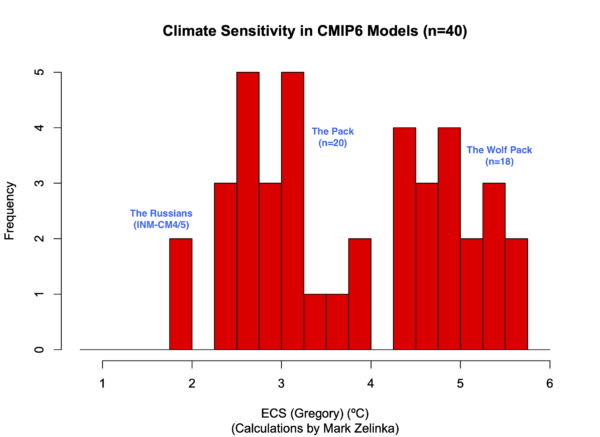
\includegraphics{fig/Gavin_2020_cmip6_ecs.png}

\href{http://www.realclimate.org/index.php/archives/2019/11/sensitive-but-unclassified/}{Gavin (2019) RealClimate (Part 1)}

\href{http://www.realclimate.org/index.php/archives/2020/06/sensitive-but-unclassified-part-ii/}{Gavin (2020) RealClimate (Part 2)}

\hypertarget{gcm-free-approach}{%
\section{GCM free Approach}\label{gcm-free-approach}}

\emph{Memo}

\begin{itemize}
\tightlist
\item
  GCM free approach
\end{itemize}

The atmosphere is a complex system involving turbulent
processes operating over a wide range of scales starting
from millimeters at the Kolmogorov dissipation scale up
to the size of the Earth, spanning over 10 orders of magni-
tudes in space.

The dynamics are sensitive to initial conditions and there are
deterministic predictability limits that
are roughly equal to the eddy turn-over time (lifetime) of
structures.

For planetary scale structures in the atmosphere,
the overall deterministic prediction limit of about 10 days
corresponds to the scaling transition timescale τ w from the
weather regime to the macroweather regime.

The atmospheric components of GCMs exhibit the same
weather-macroweather scaling transition as the atmosphere
and similar predictability limits. Beyond this horizon, the
internal variability has to be interpreted stochastically so
that a single GCM run is only one realization of the random
process; at these timescales, weather models effectively
become stochastic macroweather generators. For projec-
tions over multi-decadal timescales and beyond, multi-model
ensembles (MME) that include several models are used. The
mean of the MME is taken to obtain the deterministic forced
component of temperature variability and average out the
internal variability (Collins et al.~2013).

Emergent properties of the Earth's climate, i.e.~proper-
ties which are not specified a priori, are then inferred from
GCM simulations.

The equilibrium climate sensitivity (ECS)
is such a property; it refers to the expected temperature
change after an infinitely long time following a doubling in
carbon dioxide ( CO 2 ) atmospheric concentration.

Another is the transient climate response (TCR), which is defined
as the change in temperature after a gradual doubling of
CO 2 atmospheric concentration over 70 years at a rate of
1\% per year.

However, it is not clear whether such emer-
gent properties from computational models can be taken as
genuine features of the natural world.

The difficulty is that
each GCM has its own climate (``structural uncertainty'')
and this leads to very large discrepancies in ECS and TCR
between GCMs; this underscores the need for qualitatively
different approaches which can narrow down the properties
of the real climate directly from observations.

The ecological consequences of global warming could be dire;
therefore, better constraining climate sensitivity is of
utmost importance in order to meet the urgency of adjusting
economical and environmental policies.

Multidecadal climate projections rely almost exclusively
on deterministic global climate models (GCMs) in spite of
the fact that there are still very large structural uncertainties
between Coupled Model Intercomparison Project phase 5
(CMIP5) GCMs, i.e.~each has its own climate, rather than
the real world climate.

Climate skeptics have argued that
IPCC projections are untrustworthy precisely because they
are entirely GCM based.
While this conclusion is unwarranted, it underscores the need for
independent and qualitatively different approaches.
It is therefore significant that
the alternative GCM-free approach we present here yields
comparable results albeit with smaller uncertainty.

According to our projections made to 2100, to avert a 1.5
K warming, future emissions will be required to undergo
drastic cuts similar to RCP 2.6, for which we found a 46\%
probability to remain under the said limit; it is virtually cer-
tain that RCP 4.5 and RCP 8.5-like futures would overshoot.

Even a 2.0 K warming limit would surely be surpassed by
2100 under RCP 8.5 and probably also under RCP 4.5, with
only a 6\% chance of remaining under the limit. The safest
option remains RCP 2.6 which we project to remain under
2.0 K with very high confidence. The question remains
whether it is at all realistic given that it relies strongly on
the massive deployment of speculative negative emission
technologies.

On the other hand, our model has obvious limitations
since it assumes a linear stationary relationship between
forcing and temperature, neglecting nonlinear interac-
tions which could arise as the system evolves, as it cur-
rently warms.

In particular, so-called tipping points could
be reached in the coming century which would lead to a
breakdown of the linear model proposed. Such potential
behaviours are of critical value for improving future projections,
but they have not yet been observed with high confidence even in GCMs.

This underlines the need to exploit
paleoclimate archives to achieve a better understanding of
low-frequency natural variability, namely the transition scale
from the macroweather regime to the climate regime.

In this study, we have assumed the increased variability in the climate regime
to be strictly a result of forcing,
but internal modes of variability could also have a significant contribution
for longer timescales.

\href{https://climatenewsnetwork.net/seven-years-to-ground-zero-for-the-climate-crisis/}{Climate News Network}

\href{https://link.springer.com/article/10.1007/s00382-020-05521-x}{Climate Sensitivity article (Climate Dynamics)}
\href{pdf/Hebert_2020_Climate_Sensitivity_Estimates.pdf}{(pdf)}

\hypertarget{paleoclimate}{%
\chapter{Paleoclimate}\label{paleoclimate}}

Earth's paleoclimate history provides guidance with a precision and reliability that climate
models cannot match. Ice cores were usually the paleoclimate data source of choice for those
scientists concerned about human-made climate change. That's understandable because ice
cores provide precise data on atmospheric composition as well as climate change.
However, ice cores cover only several hundred thousand years. That sounds like a long time, but
Earth was mostly in ice ages during that time. The ice cores encompass several interglacial
periods, but none of them were much warmer than our present global temperature.
(James Hansen: Sophies Planet Ch.40)

\hypertarget{holocen-thermal-maxima}{%
\section{Holocen Thermal Maxima}\label{holocen-thermal-maxima}}

\emph{Abstract Bova}

Proxy reconstructions from marine sediment cores indicate peak temperatures in the first half of the last and current interglacial periods (the thermal maxima of the Holocene epoch, 10,000 to 6,000 years ago, and the last interglacial period, 128,000 to 123,000 years ago) that arguably exceed modern warmth1,2,3. By contrast, climate models simulate monotonic warming throughout both periods4,5,6,7. This substantial model--data discrepancy undermines confidence in both proxy reconstructions and climate models, and inhibits a mechanistic understanding of recent climate change. Here we show that previous global reconstructions of temperature in the Holocene1,2,3 and the last interglacial period8 reflect the evolution of seasonal, rather than annual, temperatures and we develop a method of transforming them to mean annual temperatures. We further demonstrate that global mean annual sea surface temperatures have been steadily increasing since the start of the Holocene (about 12,000 years ago), first in response to retreating ice sheets (12 to 6.5 thousand years ago), and then as a result of rising greenhouse gas concentrations (0.25 ± 0.21 degrees Celsius over the past 6,500 years or so). However, mean annual temperatures during the last interglacial period were stable and warmer than estimates of temperatures during the Holocene, and we attribute this to the near-constant greenhouse gas levels and the reduced extent of ice sheets. We therefore argue that the climate of the Holocene differed from that of the last interglacial period in two ways: first, larger remnant glacial ice sheets acted to cool the early Holocene, and second, rising greenhouse gas levels in the late Holocene warmed the planet. Furthermore, our reconstructions demonstrate that the modern global temperature has exceeded annual levels over the past 12,000 years and probably approaches the warmth of the last interglacial period (128,000 to 115,000 years ago).

\href{https://www.nature.com/articles/s41586-020-03155-x}{Bova (2021) Nature (Paywall)}

\hypertarget{pattern-effect}{%
\chapter{Pattern Effect}\label{pattern-effect}}

\emph{Abtract}

Our planet's energy balance is sensitive to spatial inhomogeneities in sea surface temperature and sea ice changes, but this is typically ignored in climate projections. Here, we show the energy budget during recent decades can be closed by combining changes in effective radiative forcing, linear radiative damping and this pattern effect. The pattern effect is of comparable magnitude but opposite sign to Earth's net energy imbalance in the 2000s, indicating its importance when predicting the future climate on the basis of observations. After the pattern effect is accounted for, the best-estimate value of committed global warming at present-day forcing rises from 1.31 K (0.99--2.33 K, 5th--95th percentile) to over 2 K, and committed warming in 2100 with constant long-lived forcing increases from 1.32 K (0.94--2.03 K) to over 1.5 K, although the magnitude is sensitive to sea surface temperature dataset. Further constraints on the pattern effect are needed to reduce climate projection uncertainty.

\href{https://www.nature.com/articles/s41558-020-00955-x}{Nature article (paywall)}

\hypertarget{part-elements}{%
\part{Elements}\label{part-elements}}

\hypertarget{albedo}{%
\chapter{Albedo}\label{albedo}}

Some text on Albedo

\hypertarget{atmosphere}{%
\chapter{Atmosphere}\label{atmosphere}}

\begin{verbatim}
- Emissions
    - CO2    
    - Methane
    -
- Attributing Emissions
    - Norway's Responsibility
\end{verbatim}

\hypertarget{emissions}{%
\section{Emissions}\label{emissions}}

\hypertarget{co2}{%
\subsection{CO2}\label{co2}}

\hypertarget{methane}{%
\subsection{Methane}\label{methane}}

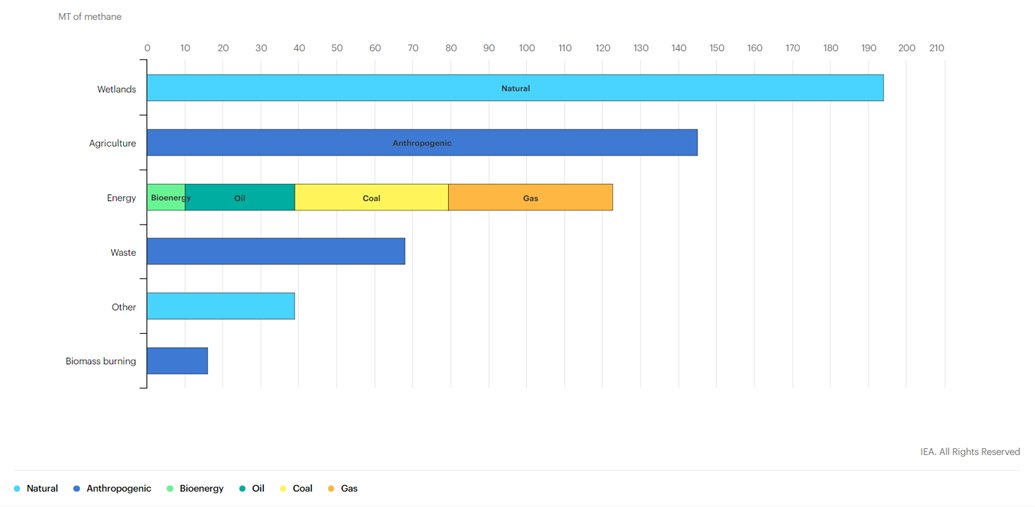
\includegraphics{fig/Methane_by_Source.jpeg}

\hypertarget{attributing-emissions}{%
\section{Attributing Emissions}\label{attributing-emissions}}

\hypertarget{norways-responsibility}{%
\subsection{Norway's Responsibility}\label{norways-responsibility}}

\begin{verbatim}
In real life responsibility is more than what is legally binding
\end{verbatim}

The emissions of CO2 that occur within Norway's territory are dwarfed by the emissions that result from combustion of all the oil and gas Norway produces. Because these fossil fuels are exported before being combusted, the emissions are allocated to the accounts of other countries. If Norway had generated electricity from the gas and then exported the electricity, for example, then emissions from that electricity generation would be allocated to Norway's accounts. There is therefore an element of artificiality associated with this allocation. It takes two to tango.

Norway's territorial emissions of CO2 were about 42 Mt in 2019, and over 1971--2019 totalled about 1.9 Gt. In comparison, emissions from Norwegian oil and gas since 1971 have been about 16 Gt. A similar amount (\textasciitilde15 Gt) will be emitted if all remaining Norwegian oil and gas resources are extracted from the continental shelf.

In 2019, emissions from Norwegian oil and gas amounted to 84 tonnes of CO2 for every person in Norway.

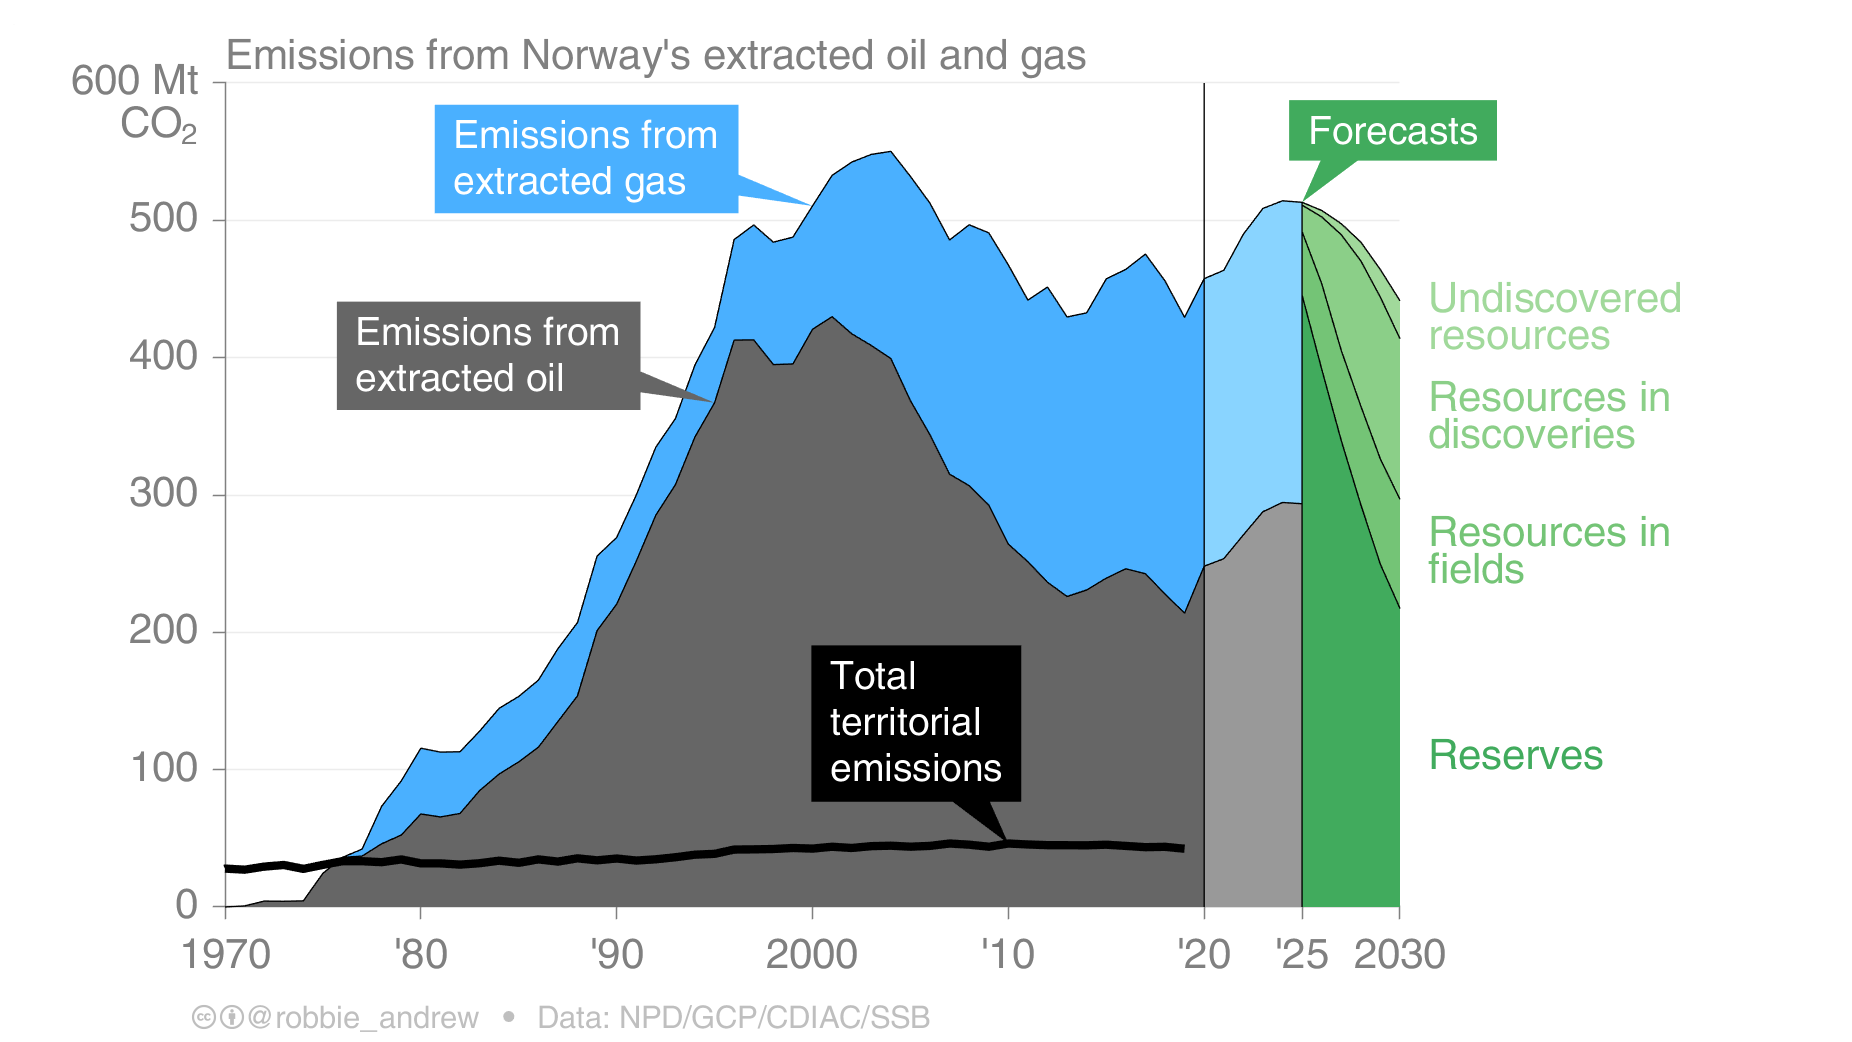
\includegraphics{fig/Emissions_extracted_Oil_Gas_Norway.png}

\href{https://folk.universitetetioslo.no/roberan/t/export_emissions.shtml}{Norways Export Emissions (Robbie Andrew)}

In Norwegian politics, there's been a very successful attempt to separate the discussion of oil policy from the discussion of climate policy. The two were never really tightly linked {[}in the country{]} until roughly the last decade, and this division has become increasingly difficult to maintain.

Norwegian politicians also haven't been alone in creating the conditions that made this division possible. They've been helped immensely by the international climate regime.

From the very beginning of international climate policy, there was this agreement that countries had to account for the emissions that they create when they burn fossil fuels. All the responsibility was placed on the demand side, not the supply side, which was very convenient for Norway.

Europe is the primary market for Norway's oil and gas. But determining the climate effects of Norwegian production is not straightforward. One study has estimated a clear climate benefit from reducing oil output, but the market is complex and the result really depends on your assumptions about how other actors will behave and how the market will evolve over time.

The big irony here is that Norway is a fairly large fossil-fuel producer, but we use relatively few fossil fuels directly in our energy use. Nearly all of our electricity has for a long time come from hydropower. In most years, we even export quite a lot of renewable electricity to our neighbors.
The only place where fossil fuels are used to directly produce energy is to run the platforms offshore. They use gas to run the turbines to get the energy needed for oil and gas production.

The government's new climate plan, which was unveiled just a few days ago, does include a number of new and more aggressive measures to reduce Norway's domestic emissions. The proposal to increase the already quite high CO2 tax on offshore emissions came as something of a surprise, and it is likely to pass even if it is currently being challenged by the industry.

However, it is important to keep in mind that this proposal only targets the production-related emissions of Norwegian oil, not the level of oil that is being extracted and exported. As such, it is in line with the historical separation between climate and oil policymaking, which tends to focus only on emissions happening within Norway and exclude any concern for the climate impact of exported oil and gas.

The Norwegian paradox has worked out fairly well up until the last few years because there has been little focus on the production of fossil fuels, and because Norway is small enough to avoid the scrutiny that some larger nations face. But this is quickly changing, both in the domestic and international political discussion.

There is now a lot more focus on the supply side of fossil fuels than 10 years ago, with several countries like Denmark announcing an end to drilling and new research showing a mismatch between planned fossil-fuel production and ideas such as a ``non-proliferation treaty'' for fossil fuels being floated. The treaty would bring the world together in agreeing to end the use of fossil fuels much like the UN came together to curb the spread of nuclear weapons.

This will make it increasingly hard for Norway to hold on to a leadership claim as long as oil production keeps being expanded into new areas.

\href{https://www.vox.com/22227063/norway-oil-gas-climate-change}{Norways Climate - Petroleum Dilemma (Bard Lahn)}

\hypertarget{forests}{%
\chapter{Forests}\label{forests}}

\hypertarget{forests-tipping-go-from-sink-to-source-of-co2-due-to-temperature-increase.}{%
\section{Forests tipping: go from sink to source of CO2 due to temperature increase.}\label{forests-tipping-go-from-sink-to-source-of-co2-due-to-temperature-increase.}}

New research shows that Earth's overheated climate will
alter forests at a global scale even more fundamentally,
by flipping a critical greenhouse gas switch in the next few decades.
The study suggests that, by 2040, forests will take up only
half as much carbon dioxide from the atmosphere as they do now,
if global temperatures keep rising at the present pace.

Global warming has contributed to thinning canopies in European forests
and to sudden die-offs of aspen trees in Colorado,
as well as insect outbreaks that are killing trees around the world.
In many places, forests are not growing back.

The data show a clear temperature limit,
above which trees start to exhale more CO2 than they can take in through photosynthesis.
The findings mark a tipping point, of sorts, at which ``the land system will act to accelerate climate change rather than slow it down,''

\href{https://insideclimatenews.org/news/13012021/forests-heat-climate-change/}{Trees From Sink to Source (InsideClimateNews)}

At present, the land provides a ``climate service'' by absorbing
around 30 per cent of the emissions caused by humans each year.

Unlike other tipping elements in the Earth system, the climate tipping point
for the terrestrial biosphere could be exceptionally close --
20-30 years away -- without action.

Plant respiration, the process by which plants produce energy for growth,
causes CO2 to be released into the atmosphere.

The `buffer' or `discount' against carbon emissions that we currently receive from the biosphere is more fragile than we previously realised.

Climate models are tools used by scientists to simulate how the world is likely to respond to greenhouse gas emissions.

However, it is worth noting that the global dataset used in the study
uses ``very few samples from tropical regions''.
This means that it is still not fully understood how tropical forests
are responding to rising temperatures.

\href{https://www.independent.co.uk/environment/climate-change/land-ecosystems-tipping-point-temperature-b1786822.html}{Independent}

\emph{Memo Duffy}

The temperature dependence of global photosynthesis and respiration
determine land carbon sink strength.
While the land sink currently mitigates \textasciitilde30\% of anthropogenic carbon emissions,
it is unclear whether this ecosystem service will persist and
what hard temperature limits, if any, regulate carbon uptake.

The mean temperature of the warmest quarter (3-month period)
passed the thermal maximum for photosynthesis during the past decade.
At higher temperatures, respiration rates continue to rise
in contrast to sharply declining rates of photosynthesis.

Under business-as-usual emissions, this divergence elicits a
near halving of the land sink strength by as early as 2040.

The difference between gross primary productivity
and total ecosystem respiration
(carbon uptake by vegetation minus carbon loss to the atmosphere)
comprises the metabolic component of the land carbon
sink {[}net ecosystem productivity (NEP){]}.

To date, land ecosystems provide a climate regulation service
by absorbing \textasciitilde30\% of anthropogenic emissions annually.
While temperature functions as a key driver
of year-to-year changes in the land carbon sink,
its temperature response is still poorly constrained at biome to global scales,
making the carbon consequences of anticipated warming uncertain.

Like all biological processes, metabolic rates for photosynthesis
and respiration are temperature dependent; they accelerate with in-
creasing temperature, reach a maximum rate, and decline thereafter.

Highly divergent land carbon sink trajectories from Earth system models.

Continued future increases in sink strength due to the CO2 fertilization.

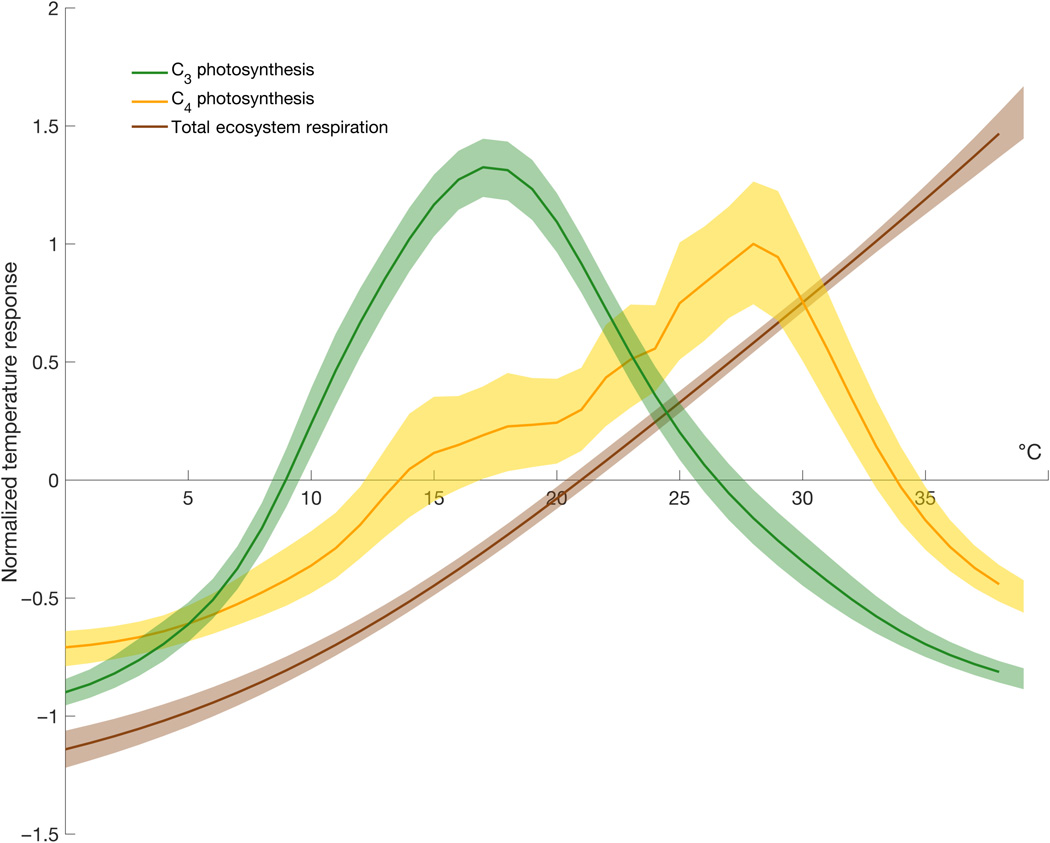
\includegraphics{fig/Photosythesis_Temp_Response.jpg}

The temperature response of global photosynthesis
shows distinct maxima at 18°C for C3 and 28°C for C4 plant systems.
In contrast to photosynthesis, respiration rates increase across
the range of ambient temperatures (up to 38°C),
with no evidence of Tmax or rate decline.
The thermal maxima of leaf and soil respiration reside at \textasciitilde60°-70°C.

Responses diverge at temperatures above Tmax.
The imbalance grows more pronounced as temperature increases.

Current climate mostly lies just below Tmax where slight increases in temperature act as
climate fertilization of land carbon uptake.
Under anticipated warming foreshadowed by historical temperature extremes and coincident
land carbon loss---however, more and more time will be spent above Tmax.
Past this threshold, the land carbon balance will first weaken and
ultimately reverse sign from carbon sink to carbon source.

25°C constitutes a powerful tipping point for the land
sink of carbon and a formidable positive climatic feedback,

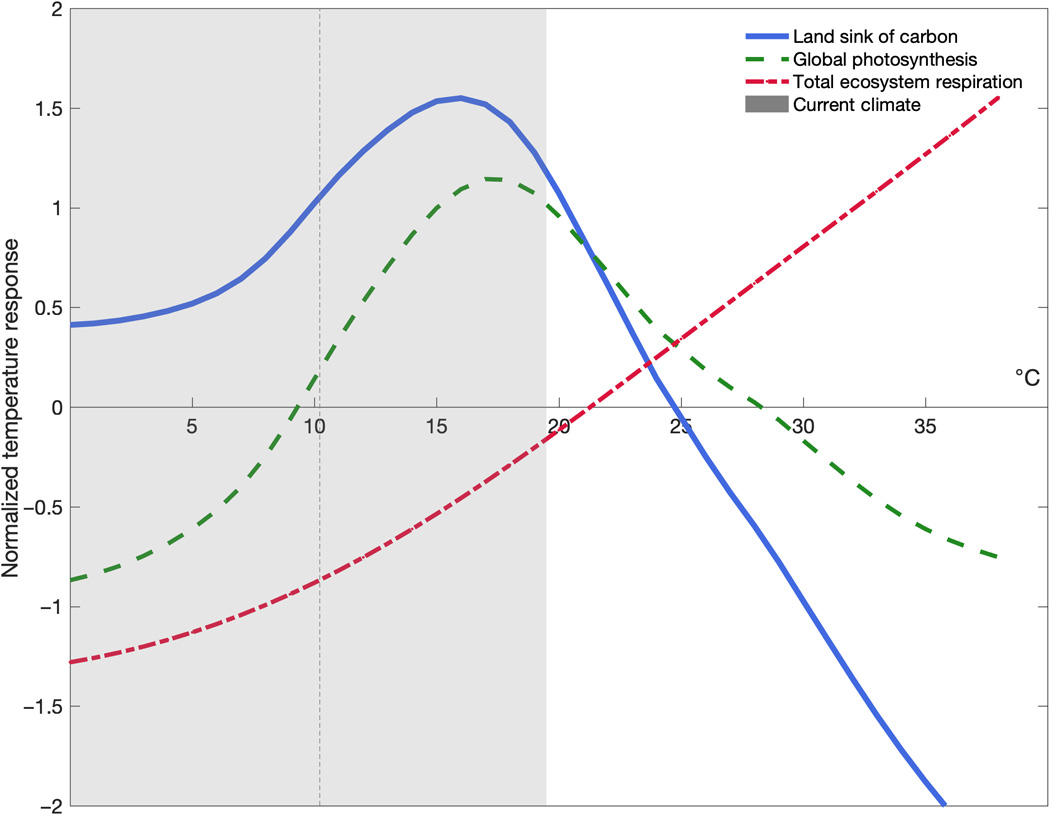
\includegraphics{fig/Land_Sink_of_Carbon.jpg}

Currently, less than 10\% of the terrestrial biosphere experiences
where land carbon uptake is degraded.
For regions that do experience these temperatures,
exposure is limited to 1 to 2 months or
constitutes areas with sparse to no vegetation.

Under business-as-usual emissions, by 2100, up to half
of the terrestrial biosphere could experience temperatures past
the treshold.

The impact of elevated temperatures on the land sink is more than a
function of cumulative area.
Biomes that cycle 40 to 70\% of all terrestrial carbon
including the rainforests of the Amazon and Southeast Asia and
the Taiga forests of Russia and Canada
are some of the first to exceed biome-specific Tmax
for half the year or more.
This reduction in land sink strength is effectively front-loaded
in that a 45\% loss occurs by midcentury,
with only an additional 5\% loss by the end of the century.
These estimates are conservative as they assume
full recovery of vegetation after temperature stress and
ignore patterns and lags in recovery.

In contrast to any CO2 fertilization effect,
anticipated higher temperatures associated with
elevated CO2 could degrade land carbon uptake.
Failure to account for this results in
a gross overestimation of climate change mitigation provided by terrestrial vegetation.

We are rapidly entering temperature regimes where biosphere productivity
will precipitously decline and
calls into question the future viability of the land sink.

\href{https://advances.sciencemag.org/content/7/3/eaay1052}{Duffy(2021) Temperature tipping point of the terrestrial biosphere}
\href{pdf/Duffy_2020_Temperature_Tipping_Point.pdf}{(pdf)}

\hypertarget{ice-sheet}{%
\chapter{Ice Sheet}\label{ice-sheet}}

\hypertarget{greenland}{%
\section{Greenland}\label{greenland}}

\emph{Abstract Noel}

Under anticipated future warming, the Greenland ice sheet (GrIS) will
pass a threshold when meltwater runoff exceeds the accumulation of snow,
resulting in a negative surface mass balance (SMB \textless{} 0) and sustained mass loss.

Here we dynamically and statistically downscale the outputs of an
Earth system model to 1 km resolution to infer that a Greenland near‐surface
atmospheric warming of 4.5 ± 0.3 °C---relative to pre‐industrial---is required
for GrIS SMB to become persistently negative.

Climate models from CMIP5 and CMIP6 translate this regional temperature change
to a global warming threshold of 2.7 ± 0.2 °C.
Under a high‐end warming scenario, this threshold may be reached around 2055,
while for a strong mitigation scenario it will likely not be passed.
Depending on the emissions scenario taken, our method estimates a 6‐13 cm sea level rise
from GrIS SMB in the year 2100.

\href{https://agupubs.onlinelibrary.wiley.com/doi/10.1029/2020GL090471}{Noel (2021) Greenland Ice Sheet Loss}
\href{pdf/Noel_2021_Greenland_Ice_Sheet_Loss.pdf}{(pdf)}

\hypertarget{antarctica}{%
\section{Antarctica}\label{antarctica}}

\hypertarget{ocean}{%
\chapter{Ocean}\label{ocean}}

Some text on Ocean

\hypertarget{permafrost}{%
\chapter{Permafrost}\label{permafrost}}

Some text on Permafrost

\hypertarget{part-policy}{%
\part{Policy}\label{part-policy}}

\hypertarget{adaptation}{%
\chapter{Adaptation}\label{adaptation}}

Climate Services may help build \emph{resilience}

\href{https://gfcs.wmo.int/}{Climate Services}

\href{https://klimaservicesenter.no/faces/desktop/index.xhtml}{Norsk KlimaServiceSenter}

\hypertarget{lagging-mitigation-lagging-adaptation}{%
\section{Lagging mitigation, lagging adaptation}\label{lagging-mitigation-lagging-adaptation}}

Given the current uncertainties around efforts to limit climate change,
the world must plan for, finance and implement climate change adaption measures
appropriate for the full range of global temperature increases or
face serious costs, losses and damages.

Adaptation -- reducing countries' and communities' vulnerability to climate change
by increasing their ability to absorb impacts and remain resilient --
is a key pillar of the Paris Agreement.
The Agreement requires all of its signatories to plan and implement adaptation measures
through national adaptation plans, studies, monitoring of climate change effects and
investment in a green future.

The Gap Report finds that such action is lagging far behind where it should be.
It finds that while nations have advanced in planning and implementation, huge gaps remain,
particularly in finance for developing countries and
bringing adaptation projects to the stage where they bring real reductions in climate risks.

The Green Climate Fund (GCF) has allocated 40 per
cent of its total portfolio to adaptation and is increasingly crowding-in private sector investment.
Another important development is the increasing momentum to ensure a sustainable financial
system.

New tools such as sustainability investment criteria, climate-related disclosure principles
and mainstreaming of climate-related risks into investment decisions can stimulate investments in
climate resilience and direct finance away from investments that increase vulnerability.

Nature-based solutions (NbS), one of the most cost-effective ways in the adaptation portfolio, has
a potential to make a big contribution to climate change adaptation, but there are few tangible
plans and limited financing available for them.
NbS are mainly used to address coastal hazards, intense precipitation, heat and
drought.

\href{https://www.unep.org/resources/adaptation-gap-report-2020}{UNEP Adaptation Report 2020}

\begin{verbatim}
Carbon Pricing
Carbon Offsets
\end{verbatim}

\hypertarget{carbon-pricing}{%
\chapter{Carbon Pricing}\label{carbon-pricing}}

\emph{Green -Abstract}

Carbon pricing has been hailed as an essential component of any sensible climate policy. Internalize the externalities, the logic goes, and polluters will change their behavior. The theory is elegant, but has carbon pricing worked in practice? Despite a voluminous literature on the topic, there are surprisingly few works that conduct an ex-post analysis, examining how carbon pricing has actually performed. This paper provides a meta-review of ex-post quantitative evaluations of carbon pricing policies around the world since 1990. Four findings stand out. First, though carbon pricing has dominated many political discussions of climate change, only 37 studies assess the actual effects of the policy on emissions reductions, and the vast majority of these are focused on Europe. Second, the majority of studies suggest that the aggregate reductions from carbon pricing on emissions are limited -- generally between 0\% and 2\% per year. However, there is considerable variation across sectors. Third, in general, carbon taxes perform better than emissions trading schemes (ETSs). Finally, studies of the EU-ETS, the oldest emissions trading scheme, indicate limited average annual reductions -- ranging from 0\% to 1.5\% per annum. For comparison, the IPCC states that emissions must fall by 45\% below 2010 levels by 2030 in order to limit warming to 1.5 degrees Celsius -- the goal set by the Paris Agreement (IPCC 2018). Overall, the evidence indicates that carbon pricing has a limited impact on emissions.

"Green -Memo*

Carbon taxes place a surcharge on fuel or energy use. In emissions trading schemes, the
government sets a ceiling or cap on the total amount of allowed emissions. Allowances are
distributed to those firms regulated by the scheme, either free of charge or by auction. Each
firm then has the right to emit up to its share of allowances. They may also trade allowances
with each other to meet their individual emission allocations. Those who emit more than their
allowance can purchase more; those that emit less can sell their excess supply, or bank it for
future use.
an
Carbon taxes and ETSs differ in a number of respects. First, carbon taxes provide certainty of
cost: the price is set by the government. Yet there is no limit on emissions, provided that
regulated entities are willing and able to pay the tax. By contrast, ETSs provide certainty of
quantity: the cap, set by the government, constitutes the upper limit on emissions. The cost
will vary, depending on the scarcity (or oversupply) of allowances, and other design features. In
practice, the distinction between the two policies is sometimes blurred (Hepburn, 2006). For
example, an ETS might have a floor price; this guaranteed price makes it resemble a tax.

First, the mismatch between the incremental effects of
carbon pricing and the demand for rapid decarbonization cannot be understated. The IPCC
states that emissions must fall by 45\% below 2010 levels by 2030 in order to limit warming to
1.5 degrees Celsius -- the goal set by the Paris Agreement (IPCC 2018). The Low Carbon
Economy Index estimates that this translates to an annual emissions reduction of 11.3\% by the
``average'' G20 nation (PwC 2019). Yet GHG emissions have risen an average of 1.5\% per year in
the last decade (UN Environment 2019, p.~iv). It is important to understand the extent to which
one of the most widely-used climate policies contributes to this goal.

Second, there is little evidence to suggest that carbon pricing promotes decarbonization
The most common outcome is fuel-switching and efficiency improvements.
Unlike policies which create pathways to decarbonization -- such as binding renewable
portfolio standards, feed in tariffs or investment in R\&D --
carbon pricing addresses emissions (flow), rather than overall concentrations of
greenhouse gases (stock).

The real work of emission control is done through regulatory instruments.
Within the EU, where nations are also part of the EU-ETS, nations without a carbon
tax reduced emissions more quickly than those with a carbon tax.

It is astonishing how little hard evidence there is on the actual performance of
carbon pricing policies using ex-post data.
Tthe overall effect on reductions for both types of policy is
quite small, generally between 0-2\% per annum.
Norway, Sweden and Denmark were early
adopters, implementing some of the first carbon taxes in 1991-92.
EU-ETS was the first compulsory emissions trading scheme, beginning in 2005.

The single study of California cap and trade scheme
estimates that between 24\%-43\% of emissions from electricity generation were shifted out of
state to avoid carbon pricing regulations.

The drivers of these modest reductions are incremental solutions: fuel switching,
enhanced efficiency, and reduced consumption of fuels.
These actions, though useful on the margins, fall well short of
the societal transformations identified needed.

A common rejoinder is that carbon prices simply aren't high enough to generate substantial
emissions reductions.
Indeed, low prices are pervasive; the vast majority of carbon prices are
well below even the most conservative estimates of the ``social cost of carbon'' (SCC).

Given the prevalence of low prices, it is particularly important to consider the few jurisdictions
with carbon prices at or near the SCC.
Sweden has the highest carbon price in the world.
Studies range in their reduction estimates from 0\%-17\% per year, with the upward
bound being an outlier among all 37 studies.
In 2019, Finnish taxes on transport fuels were at \$68 per ton, and \$58 per ton for
all other fossil fuels.
Emissions reductions there are estimated to be between 0\%-1.7\%
The other two jurisdictions with high carbon taxes are
Switzerland (\$99 per ton in 2019) and Lichtenstein (\$99 per ton in 2019
, No estimates of their effects on emissions).

It may be the case that pricing will work better after a certain threshold is surpassed. Indeed,
Aydin and Esen find that energy taxes, including CO2 taxes, only reduce emissions after
surpassing 2.2\% of GDP (2018). Yet after nearly four decades of experience with carbon pricing,
the empirical evidence to date suggests that low prices are a feature of this policy, rather than a
bug. More worrisome is the fact that even those nations with high prices have relatively
modest reductions.

A problem for carbon pricing concerns leakage, which occurs when economic
activity subject to carbon pricing shifts to a jurisdiction without similar regulations. This
problem is pervasive in environmental regulation, driven by variation in policy stringency.
To the extent that leakage occurs, but is excluded from the studies examined here, emissions
reductions may be overestimated.

Offsets can have two possible impacts on overall reductions. First, to the extent that offsets are
not additional, their use will decrease the actual reductions achieved through a carbon pricing
policy.
To date, offsets have been an important component of most ETSs.

\href{https://iopscience.iop.org/article/10.1088/1748-9326/abdae9/meta}{Green(2021) Carbon Pricing Ex-Post}
\href{pdf/Green_2021_Carbon_Pricing_Ex-Post.pdf}{(pdf)}

\hypertarget{carbon-offsets}{%
\chapter{Carbon Offsets}\label{carbon-offsets}}

Carbon offset schemes allow individuals and companies to invest in environmental projects around the world in order to balance out their own carbon footprints. The projects are usually based in developing countries and most commonly are designed to reduce future emissions. This might involve rolling out clean energy technologies or purchasing and ripping up carbon credits from an emissions trading scheme. Other schemes work by soaking up CO2 directly from the air through the planting of trees.

\begin{itemize}
\tightlist
\item
  Selling Indulgencies*
  George Monbiot famously compared carbon offsets with the ancient Catholic church's practice of selling indulgences: absolution from sins and reduced time in purgatory in return for financial donations to the church.
  Just as indulgences allowed the rich to feel better about sinful behaviour without actually changing their ways, carbon offsets allow us to buy complacency, political apathy and self-satisfaction.
\end{itemize}

\emph{Additionality}
the key issue for anyone who does want to offset is whether the scheme you're funding actually achieves the carbon savings promised. This boils down not just to the effectiveness of the project at soaking up CO2 or avoiding future emissions. Effectiveness is important but not enough. You also need to be sure that the carbon savings are additional to any savings which might have happened anyway.
The problem is that it's almost impossible to prove additionality with absolute certainly, as no one can be sure what will happen in the future, or what would have happened if the project had never existed.

Partly because of the difficulty of ensuring additionality, many offset providers guarantee their emissions savings. This way, if the emissions savings don't come through or they turn out to be ``non-additional'', the provider promises to make up the loss via another project.

As the offset market grows, some offset companies have enough capital to invest in projects speculatively: they fund an offset project and then sell the carbon savings once the cuts have actually been made. This avoids the difficulty of predicting the future -- and also avoids the claim that a carbon cut made some years in the future is worth less than a cut made now.

These kinds of guarantees and policies provide some reassurances, but do they mean anything in the real world? Without actually visiting the offset projects ourselves, how can individuals be sure that the projects are functioning as they should?

Even if offset projects do work as advertised, some environmentalists argue that they're still a bad idea. If we're to tackle climate change, they argue, the projects being rolled out by offset companies should be happening anyway, funded by governments around the world, while companies and individuals reduce their carbon footprints directly. Only in this way -- by doing everything possible to make reductions everywhere, rather than polluting in one place and offsetting in another -- does the world have a good chance of avoiding runaway climate change, such critics claim.

\emph{Market Standards}
To try and answer these questions, the voluntary offset market has developed various standards, which are a bit like the certification systems used for fairly traded or organic food. These include the Voluntary Gold Standard (VGS) and the Voluntary Carbon Standard (VCS).
Offsets with these standards offer extra credibility, but that still doesn't make them watertight. Heather Rogers, author of Green Gone Wrong, visited a number of offset schemes in India and found all kinds of irregularities.

\emph{Offset Price}
Many people are confused by the low prices of carbon offsets. If it's so bad for the environment to fly, can a few pounds really be enough to counteract the impact? The answer is that, at present, there are all kinds of ways to reduce emissions very inexpensively. After all, a single low-energy lightbulb, available for just £1 or so, can over the space of six years save 250kg of CO2 -- equivalent to a short flight. That's not to say that offsetting is necessarily valid, or that plugging in a low-energy lightbulb makes up for flying. The point is simply that the world is full of inexpensive ways to reduce emissions. In theory, if enough people started offsetting, or if governments started acting seriously to tackle global warming, then the price of offsets would gradually rise, as the low-hanging fruit of emissions savings -- the easiest and cheapest ``quick wins'' -- would get used up.

Another frequent point of confusion about the cost of offsetting is that different offset companies quote different prices for offsetting the same activity. There are two reasons for this. First, there are various ways of estimating the precise impact on climate change of certain types of activity -- including flying, which affects global temperature in various different ways. Second, different types of offset project will inevitably have different costs -- especially given that projects may be chosen not just for the CO2 impacts but for their broader social benefits.

\href{https://www.theguardian.com/environment/2011/sep/16/carbon-offset-projects-carbon-emissions\#:~:text=Carbon\%20offset\%20schemes\%20allow\%20individuals,designed\%20to\%20reduce\%20future\%20emissions.}{Duncan Clark (Guardian 2011): Complete Guide to Carbon Offsetting}

\hypertarget{market-upscaling}{%
\section{Market Upscaling}\label{market-upscaling}}

Carney presented plans at the virtual Davos meeting of global business and political leaders on Wednesday evening for vast increases in the number of carbon offsets sold, aiming to expand the market from about \$300m at present to between \$50bn and \$100bn a year.

He told the conference that he ``categorically rejected'' criticism that offsets were greenwash. Companies buying offsets in the market would be subject to scrutiny, and must have clear plans to reach net zero, ``not something written on the back of a napkin'', he said, but would need offsets to fulfil their plans.

``This is bringing those companies into a formal system,'' he said. ``This is about maximising the use of a very limited {[}global{]} carbon budget. This is complementary {[}to companies taking action to reduce their own emissions{]} and is one piece of the puzzle. We do need this market.''

The leaders of two UK environmental charities have written to Mark Carney, the UN climate envoy and former governor of the Bank of England, to raise concerns over the blueprint for carbon offsetting that could result in billions of new carbon credits being sold around the world.

Campaigners say system risks becoming greenwashing exercise unless loopholes closed.

The markets are used as a cover by companies that wish to give the appearance of working towards net zero emissions but prefer buying cheap credits to the more difficult task of cutting their emissio

This initiative risks setting a terrible example ahead of the critical carbon market negotiations at the global climate summit in Glasgow later this year. {[}It{]} seems to have ignored past failures of offsetting schemes to guarantee emission cuts. At the same time, it assumes that the natural world has unlimited potential to absorb climate-wrecking emissions. It fails to acknowledge that the most important thing companies must do is to reduce their own emissions and use of fossil fuels.

Carney's scheme will serve as a giant get-out-of-jail-free card for polluting companies.

There is a danger that it becomes a large international greenwashing exercise, creating a market with low standards but high PR value,

\href{https://www.theguardian.com/environment/2021/jan/27/green-groups-raise-concerns-over-carney-carbon-credits-plan}{Guardian on Carney Offsets}

\begin{quote}
If you scale a bad thing, it doesn't matter how big you make it, it's still bad.
\end{quote}

As Mark Carney presented the world's top political and business leaders with a blueprint to scale up the voluntary carbon market on Wednesday, campaigners warned key criteria to improve environmental integrity were missing.

With carbon neutrality pledges becoming the benchmark for climate ambition, businesses around the world are looking to offset the emissions they cannot cut and for cheaper ways to meet their climate goals.

Its report identified ways to bring coherence to what is currently a fragmented market. But it said little on how to ensure projects financed through the market deliver genuinely additional emissions reductions.

An open letter to Carney signed by 47 researchers, academics and campaigners ahead of the launch accused the initiative of trying to ``minimise the cost of compliance for private corporations'' at the cost of environmental integrity.

An independent process driven by civil society should define what constitute a quality offset to avoid the private sector self-regulating.

Sequestrating carbon in ecosystems should not replace real emissions cuts.
We need to sequester past emissions that are already in the atmosphere whereas offsetting by definition is about future emissions. The whole point of an offset is that an entity keeps emitting. There is a striking lack of binding and credible measures to actually prioritise emissions reductions.

The biodiversity co-benefits that result from the voluntary carbon market are ``a strong assumption'' with no evidence.

It's important not to forget the huge flows of finance currently facilitating the drivers of biodiversity loss - warning against the market being perceived as an adequate substitute to conservation.

\href{https://www.climatechangenews.com/2021/01/27/carneys-carbon-offset-taskforce-ducks-environmental-integrity-questions/}{ClimateChangeNews}

\emph{Memo TSVCM Report}

Chaired by Bill Winters, group chief executive of Standard Chartered, and sponsored by the Institute of International Finance (IIF), the taskforce includes some of the world's most polluting companies: airline easyJet, plane manufacturer Boeing, oil giants BP, Shell and Total, and steel producer Tata Steel. No green groups are represented among its members.

The need for climate action, and tools to
mobilize finance for the low-carbon and
resilient transition, grows more urgent by the
day. To achieve the Paris goals to limit global
warming to 1.5 degrees Celsius, the global
community needs to reach net-zero emissions
by no later than 2050. This will require a
whole-economy transition---every company,
every bank, every insurer and investor
will have to adjust their business models,
develop credible plans for the transition, and
implement them.

Many companies, especially in hard-to-
abate sectors, will need to offset emissions
as they achieve their decarbonization goals,
creating a surge in demand for credible
offsets.

To facilitate this global
decarbonization there is a need for a large,
transparent, verifiable and robust voluntary
carbon market, one that promotes genuine
action of high environmental integrity.

Along with the carbon avoided, reduced, or
removed, the scaling up of markets has the
further potential to help support financial
flows to the Global South, as activities and
projects in these countries can provide a cost-
effective source of these carbon-emission
reductions. Voluntary carbon markets can
also play a critical role in scaling down cost
curves for emerging climate technologies,
bringing these technologies to market earlier,
and allowing them to be used in direct
decarbonization efforts.

The Taskforce has found
six key areas where efforts are required
to achieve a large, transparent, verifiable,
and robust voluntary carbon market;
these themes are establishing core carbon
principles, core carbon reference contracts,
infrastructure, offset legitimacy, market
integrity, and demand signaling.

!! Direct
emissions reductions by corporates must
be the priority, with appropriate offsetting
playing an important complementary role
to accelerate climate mitigation action.

\href{https://www.iif.com/tsvcm}{Taskforce on Scaling Voluntary Carbon Markets}
\href{pdf/TSVCM_2021_Scaling_Carbon_Markets.pdf}{(pdf)}

\hypertarget{css---carbon-capture-and-storage}{%
\chapter{CSS - Carbon Capture and Storage}\label{css---carbon-capture-and-storage}}

\emph{Tyndall Report:}

CCS, as the technology is known, is designed to
strip out carbon dioxide from the exhaust gases of industrial processes.
These include gas- and coal-fired electricity generating plants, steel-making,
and industries including the conversion of natural gas to hydrogen,
so that the gas can then be re-classified as a clean fuel.

The CO2 that is removed is converted into a liquid and pumped underground
into geological formations that can be sealed for generations
to prevent the carbon escaping back into the atmosphere.

It is a complex and expensive process, and many of the schemes proposed in the 1990s
have been abandoned as too expensive or too technically difficult.

Currently (2020) there are only 26 CCS plants operating globally,
capturing about 0.1\% of the annual global emissions from fossil fuels.

Ironically, 81\% of the carbon captured to date has been used to
extract more oil from existing wells by pumping the captured carbon into the ground
to force more oil out.
This means that captured carbon is being used to extract oil that
would otherwise have had to be left in the ground.

CCS features prominently in many energy and climate change scenarios,
and in strategies for meeting climate change mitigation targets.

It is the cumulative emissions from each year between now and 2030 that will
determine whether we are to achieve the Paris 1.5°C goal.
With carbon budgets increasingly constrained we cannot expect
CSS to make a meaningful contribution to 2030 climate targets.

\hypertarget{css-will-not-work-as-planned-and-is-a-dangerous-distraction}{%
\subsection{CSS will not work as planned and is a dangerous distraction}\label{css-will-not-work-as-planned-and-is-a-dangerous-distraction}}

Instead of financing a technology they can neither develop in time
nor make to work as claimed,
governments should concentrate on scaling up proven technologies
like renewable energies and energy efficiency.

The technology has not lived up to expectations.
Instead of capturing up to 95\% of the carbon from any industrial process,
rates have been as low as 65\% when they begin and have only gradually improved.

\href{https://climatenewsnetwork.net/carbon-capture-and-storage-wont-work-critics-say/}{CCS won't work (ClimateNewsNetwork)}

Global operational CCS capacity is currently 39MtCO2 per year,
this is about 0.1\% of annual global emissions from fossil fuels.

There are just 26 operational CCS plants in the world,
with 81\% of carbon captured to date used to extract more oil
via the process of Enhanced Oil Recovery {[}EOR{]}, and at this stage
CCS planned deployment remains dominated by EOR.
Financing of these CCS projects has relied on the increased revenue from EOR,

CCS is not capable of operating with zero emissions.
Many projections assume a capture rate for CCS of 95\%, however,
capture rates at that level are unproven in practice.

Current capacity in the energy sector is just 2.4 MtCO 2 a year.
This compares to the International Energy Agency's (IEA) estimate of 310 MtCO 2 a year in the
energy sector by 2030, an increase of 129 times from today.

Reliance on CCS is not a solution to the climate emergency.

\href{https://foe.scot/resource/report-carbon-capture-storage-energy-role/}{Tyndall Centre Report}
\href{pdf/Tyndall_2020_CCS-Summary.pdf}{(pdf Summary)}
\href{pdf/Tyndall_2020_CCS-Report.pdf}{(pdf Report)}

\emph{But the industry do not agree:}

When CCS was first touted, it was seen as a way of cleaning up
electricity generated by fossil fuels, in particular those burning coal.
But now it is clear it can play a key role in cleaning up other industries.

The opposition to CCS technology from some campaigners seems
driven by a hatred of fossil fuel companies that is
preventing a level-headed understanding of how we can stop climate change.

\href{https://www.theguardian.com/environment/2021/jan/16/carbon-capture-vital-meeting-climate-goals-scientists-cut-emissions}{Industry Response to Tyndall Report}

\hypertarget{css-and-dac-cause-more-damage-than-good}{%
\section{CSS and DAC cause more Damage than Good}\label{css-and-dac-cause-more-damage-than-good}}

Spending money on carbon capture and storage or use (CCS/U) and synthetic direct air capture and storage and use (SDACCS/U) increases carbon dioxide equivalent (CO2e) emissions, air pollution, and costs relative to spending the same money on clean, renewable electricity replacing fossil or biofuel combustion.

The low net capture rates are due to uncaptured combustion emissions from natural gas used to power the equipment, uncaptured upstream emissions, and, in the case of CCU, uncaptured coal combustion emissions. Moreover, the CCU and SDACCU plants both increase air pollution and total social costs relative to no capture. Using wind to power the equipment reduces CO2e relative to using natural gas but still allows air pollution emissions to continue and increases the total social cost relative to no carbon capture. Conversely, using wind to displace coal without capturing carbon reduces CO2e, air pollution, and total social cost substantially. Further, using wind to displace coal reduces more CO2e than using the same wind to power the capture equipment. As such, spending money on wind powering carbon capture always increases CO2e compared with spending on the same wind replacing fossil fuels or biofuels. In sum, CCU and SDACCU increase or hold constant air pollution health damage and reduce little carbon before even considering sequestration or use leakages of carbon back to the air. Spending on capture rather than wind replacing either fossil fuels or bioenergy always increases CO2e, air pollution, and total social cost substantially. No improvement in CCU or SDACCU equipment can change this conclusion while fossil power plant emissions exist, since carbon capture always incurs an equipment cost never incurred by wind, and carbon capture never reduces, instead mostly increases, air pollution and fuel mining, which wind eliminates. Once fossil power plant emissions end, CCU (for industry) and SDACCU social costs need to be evaluated against the social costs of natural reforestation and reducing nonenergy halogen, nitrous oxide, methane, and biomass burning emissions.

\href{https://research.american.edu/carbonremoval/2019/11/13/jacobson-mark-2019-why-carbon-capture-and-direct-air-capture-cause-more-damage-than-good-to-climate-and-health/}{Jakobsen (2019)}

\hypertarget{scc---social-costs-of-carbon}{%
\chapter{SCC - Social Costs of Carbon}\label{scc---social-costs-of-carbon}}

\begin{verbatim}
The most important number you have never heard of
    Greenstone Testimony
    Greenstone Estimating SCC
    Greenstone Updating SCC     
Current prices far below SCC
\end{verbatim}

SCC: The straw that stirs the drink

The dollar value that future populations and governments around the
world would be willing to pay to avoid experiencing climate change.

\begin{quote}
If you could see dimly into the future---which you can!---and calculate in dollars the benefits of actions preventing utter destruction and chaos, what would you call this price?
You might call it ``the alpha price,'' the price of having a safe future.
\end{quote}

The s̶o̶c̶i̶a̶l̶ ̶c̶o̶s̶t̶ ̶o̶f̶ ̶c̶a̶r̶b̶o̶n̶ alpha price is a regulatory tool (yawn) that addresses an important disparity, which is the difference between market prices for fossil fuels and the value of the damage they inflict on the world. By calculating the alpha price\ldots{}
and using it as a ``benefit'' in cost-benefit analyses, government can make sure that they truly understand the costs and benefits of new policies. They ensure that demonstrably incorrect market prices for fossil fuels are not obscuring the real benefits of action.
t's a complicated thing, calculating the alpha price, which brings us to the question of how bureaucratic inertia and professional conventions perpetuate thinking we don't need anymore.
Hold your breath, we're free-diving now deep into the bowels of regulatory bureaucracy.
Which brings us to the punchline: Is there a better way to bring about a net-zero, safe future without even relying on an alpha price? Is applying a cost-benefit analysis to climate change itself a part of the bureaucratic and professional conventions that are holding back climate progress? Maybe! That's why(I think!) \citet{noahqk} et al have given us Near-Term to Net-Zero and (I think) why \citet{GernotWagner}
et al have given us declining CO2 price paths.
(Eric Roston, twitter thread).

\hypertarget{the-most-important-number-you-have-never-heard-of}{%
\section{The most important number you have never heard of}\label{the-most-important-number-you-have-never-heard-of}}

\hypertarget{greenstone-testimony}{%
\subsection{Greenstone Testimony}\label{greenstone-testimony}}

\begin{itemize}
\tightlist
\item
  The social cost of carbon (SCC) is the cost to society of polluting an additional ton of CO2.
  The SCC enables regulators to account for potential benefits to society through lower carbon
  emissions and also points towards the optimal price on carbon required to address excess
  greenhouse gas emissions. The US government SCC was approximately \$50 per ton of CO2
  as of 2016, using a discount rate of 3\%.
\end{itemize}

Since its inception, the SCC has been used in roughly 150 federal regulations that cover energy
efficiency, forest conservation, fuel-economy standards, and emissions performance standards.
Indeed, in many cases the SCC was instrumental in passing these regulations, offering relevant
agencies a reliable, transparent tool to calculate the full benefits the new rules would offer to
society. All told, a recent paper calculated, federal regulations written to include the SCC in the
US have more than \$1 trillion of benefits.

When one considers the possibility of larger-than-
expected temperature changes for a given change in emissions, sea level rise in short time
periods, physical ``tipping points'', and human responses like mass migration, then the case for a
low discount rate appears strong.

The broader point is that global
interest rates have declined since the SCC was set and, even setting aside the risk characteristics
of payoffs from climate mitigation investments, there is a solid case that the discount rates
currently used to calculate the SCC may be too high.

When the US accounts for the full global benefits of reducing
our emissions, this incentivizes reciprocal climate policies in other countries, like China and
India, that reduces their emissions which benefits the US.

The use of a SCC that only
considers domestic benefits is very likely to deprive the United States of emissions reductions in
the United States that would protect us from more virulent climate change

Climate Impact Lab (CIL) aims to produce the
world's first empirically derived estimate of the social cost of carbon

CIL's core findings to date have been in the mortality sector. Climate change has a demonstrable
impact on mortality rates, as extreme temperatures, both hot and cold, affect health outcomes
such as heat stroke and cardiovascular disease. Using data from forty countries and statistical
methods to account for the benefits and costs of adaptation, we estimate the full mortality risk
due to climate change to be an additional 85 deaths per 100,000 in 2100.
This increase in the global mortality rate is more than the mortality rate associated with
all infectious diseases in 2018.

The elevated mortality risk equates to a monetary cost of \$23.6
per metric ton of carbon emitted today when using the same assumptions that underlie the
Obama SCC calculation. In other words, we estimate the partial social cost of carbon,
accounting for costs to human mortality alone, to be at least \$23.6 per ton.

The Obama administration's estimate of the SCC assumed that society is
risk neutral, that is, we are not willing to pay a premium to avoid uncertainty. If the more
realistic assumption that society is risk averse were introduced, then the estimated SCC would be
higher, likely substantially so, than the \$50 per metric ton of CO 2 discussed in the previous
section. Similarly, there is a good case for scaling the damages from the CIL's research upwards
to reflect the risk aversion that characterizes individuals' choices in their own lives.

While Accra, Ghana will see an increase in the full mortality
risk of 160 per 100,000 due to climate change in 2100, Oslo, Norway will experience a decline in
the full mortality risk of 230 per 100,000 due to warmer winters.
Climate change
will leave some regions as winners and others as losers both around the globe and within the
United States.

Climate impacts vary considerably
across locations. While northern latitudes will experience net savings due to reduced heating
needs, increased cooling demand will lead to large increases in many areas of the tropics.

Within the United States, I find that rural
areas will be hard-hit. My co-author and I estimate that with a high emissions scenario 18 , rising
temperatures will reduce 2050 corn acreage by 94\% and soybean acreage by 98\% when
compared to levels in 2002. The lost corn and soybean production will not be replaced by
increased production of any crop currently grown in the US: as returns to agriculture decline in
connection with climate change, farmers will seek to shift land use toward different crops and
non-agricultural options. It will effectively bring an end to the more than 150-year tradition of
farming as we know it in the US corn-belt that encompasses great swatches of Iowa, Nebraska,
and Illinois.

The uneven distribution of climate damages means that the very mitigation of climate change is a
pursuit of environmental justice.

\href{http://www.impactlab.org/news-insights/michael-greenstone-testifies-on-the-economic-effects-of-climate-change/}{Michael Greenstone testimony}
\href{pdf/Greenstone_2019_Testimony.pdf}{(pdf)}

\hypertarget{greenstone-estimating-scc-mit-ceepr-wp-2011-006}{%
\subsection{Greenstone Estimating SCC (MIT CEEPR WP 2011-006):*}\label{greenstone-estimating-scc-mit-ceepr-wp-2011-006}}

For 2010, the central value of the
SCC is \$21 per ton of CO 2 emissions and sensitivity analyses are to be conducted
at \$5, \$35, and \$65 (2007\$). This paper summarizes the methodology and
process used to develop the SCC values.

The 2009-2010 interagency process that developed these SCC values was the first U.S. federal
government effort to promote consistency in the way that agencies calculate the social benefits of
reducing CO 2 emissions in regulatory impact analyses. 4 Prior to 2008, reductions in CO 2
emissions were not valued in federal benefit--cost analyses.

\emph{IAMs}

Analysts face a number of significant challenges when attempting to quantify the economic
impacts of CO 2 emissions. In particular, analysts must make assumptions about four main steps
of the estimation process: (1) the future emissions of greenhouse gases; (2) the effects of past and
future emissions on the climate system; (3) the impact of changes in climate on the physical and
biological environment; and, (4) the translation of these environmental impacts into economic
damages. Integrated assessment models (IAMs) have been developed to combine these steps
into a single modeling framework; the word ``integrated'' refers to the fact that they integrate
knowledge from science and economics. However, they gain this advantage at the expense of a
more detailed representation of the underlying climatic and economic systems.

The IAMs translate emissions into changes in atmospheric greenhouse gas concentrations,
atmospheric concentrations into changes in temperature, and changes in temperature into
economic damages.

The emissions projections used in the models are based on specified socio-
economic (GDP and population) pathways. These emissions are translated into concentrations
using the carbon cycle built into each model, and concentrations are translated into warming
based on each model's simplified representation of the climate and a key parameter, climate
sensitivity. Finally, transforming the stream of economic damages over time into a single value
requires judgments about how to discount them.

(DICE-PAGE-FUND differences discussed in paper omitted here)

Overall, the power of the IAMs is that they offer guidance to the incredibly complex question of
what an extra ton of greenhouse damages will do to human wellbeing. This is no small task and
this is what makes them so appealing. However, the results are highly dependent on a series of
assumptions that cannot easily be verified.

On Discount Rates:

\emph{Historically Observed Interest Rates}

\emph{Ramsey Equation}

Ramsey discounting also provides a useful framework to inform the choice of a discount rate.
Under this approach, the analyst applies either positive or normative judgments in selecting
values for the key parameters of the Ramsey equation: η (coefficient of relative risk aversion or
elasticity of the marginal utility of consumption) and ρ (pure rate of time preference). 18 These
are then combined with g (growth rate of per-capita consumption) to equal the interest rate at
which future monetized damages are discounted: ρ + η·g.

Most papers in the climate change literature adopt values for η in the range of 0.5 to 3, although
not all authors articulate whether their choice is based on prescriptive or descriptive reasoning. 19
Dasgupta (2008) argues that η should be greater than 1 and may be as high as 3, since η equal to
1 suggests savings rates that do not conform to observed behavior. With respect to the pure rate
of time preference, most papers in the climate change literature adopt values for ρ in the range of
0 to 3 percent per year. The very low rates tend to follow from moral judgments involving
intergenerational neutrality. Some have argued that to use any value other than ρ = 0 would
unjustly discriminate against future generations (e.g., Arrow et al.~1996, Stern et al.~2006).
However, even in an inter-generational setting, it may make sense to use a small positive pure
rate of time preference because of the small probability of unforeseen cataclysmic events (Stern
et al.~2006).

Some economists and non-economists have argued for constant discount rates below 2 percent
based on the prescriptive approach. When grounded in the Ramsey framework, proponents of
this approach have argued that a ρ of zero avoids giving preferential treatment to one generation
over another. The choice of η has also been posed as an ethical choice linked to the value of an
additional dollar in poorer countries compared to wealthier ones. Stern et al.~(2006) applies this
perspective through his choice of ρ = 0.1 percent per year η = 1, yielding an annual discount rate
of 1.4 percent when combined with the growth rate. Recently, Stern (2008) revisited the values
used in Stern et al.~(2006), stating that there is a case to be made for raising η due to the amount
of weight lower values place on damages far in the future (over 90 percent of expected damages
occur after 2200 with η = 1).

If there is a persistent element to the uncertainty in the discount rate (e.g., the
rate follows a random walk), then it will result in an effective (or certainty-equivalent) discount
rate that declines over time. Consequently, lower discount rates tend to dominate over the very
long term

\emph{Updating 2021 - \$125 - Abstract}

This paper outlines a two-step process to return the United States government's
Social Cost of Carbon (SCC) to the frontier of economics and climate science.
The first step is to implement the original 2009-2010 Inter-agency Working
Group (IWG) framework using a discount rate of 2\%. This can be done
immediately and will result in an SCC for 2020 of \$125. The second step is to
reconvene a new IWG tasked with comprehensively updating the SCC over the
course of several months that would involve the integration of multiple recent
advances in economics and science. We detail these advances here and provide
recommendations on their integration into a new SCC estimation framework.

\href{pdf/Greenestone_2011_Estimating_SCC.pdf}{Michael Greenstone (2011) Estimatiung SCC (pdf)}

\hypertarget{greenstone-updating-scc}{%
\subsection{Greenstone: Updating SCC}\label{greenstone-updating-scc}}

In many respects, the SCC is the ``straw that stirs the drink'' for most domestic climate
policies, determining in some cases whether or not regulatory action can proceed.

A defining feature of the best new (after 2010) research is that it relies on large-scale data
sets, rather than assumptions that are often unverifiable.

New estimates for two of three recently studied SCC
sectors (mortality and agriculture) indicate substantially larger damages from CO 2 ,
suggesting that the SCC, as settled in 2013, is too low.
Climate change is projected to disproportionately
harm today's poorest populations, exacerbating concerns about environmental justice.

The Biden administration can initiate the first step immediately
and simply involves implementing the IWG's approach again with a discount rate of no
higher than 2 percent, which reflects profound changes in international capital markets
that make the current values difficult to justify. At a discount rate of 2\% the SCC in
2020 is \$125.

There are seven ``ingredients'' necessary to construct the SCC. The first four are often
referred to as ``modules'' :

\begin{verbatim}
1. A socioeconomic and emissions trajectory, which predicts how the global  
economy and CO 2 emissions will grow in the future;  
2. A climate module, which measures the effect of emissions on the climate;  
3. A damages module, which translates changes in climate to economic  
damages; and  
4. A discounting module, which calculates the present value of future  
damages.  
\end{verbatim}

In addition, there are three cross-cutting modeling decisions
that affect the entire process:

\begin{verbatim}
1. Whether to include global or instead only domestic climate damages;  
2. How to value uncertainty; and  
3. How to treat equity.  
\end{verbatim}

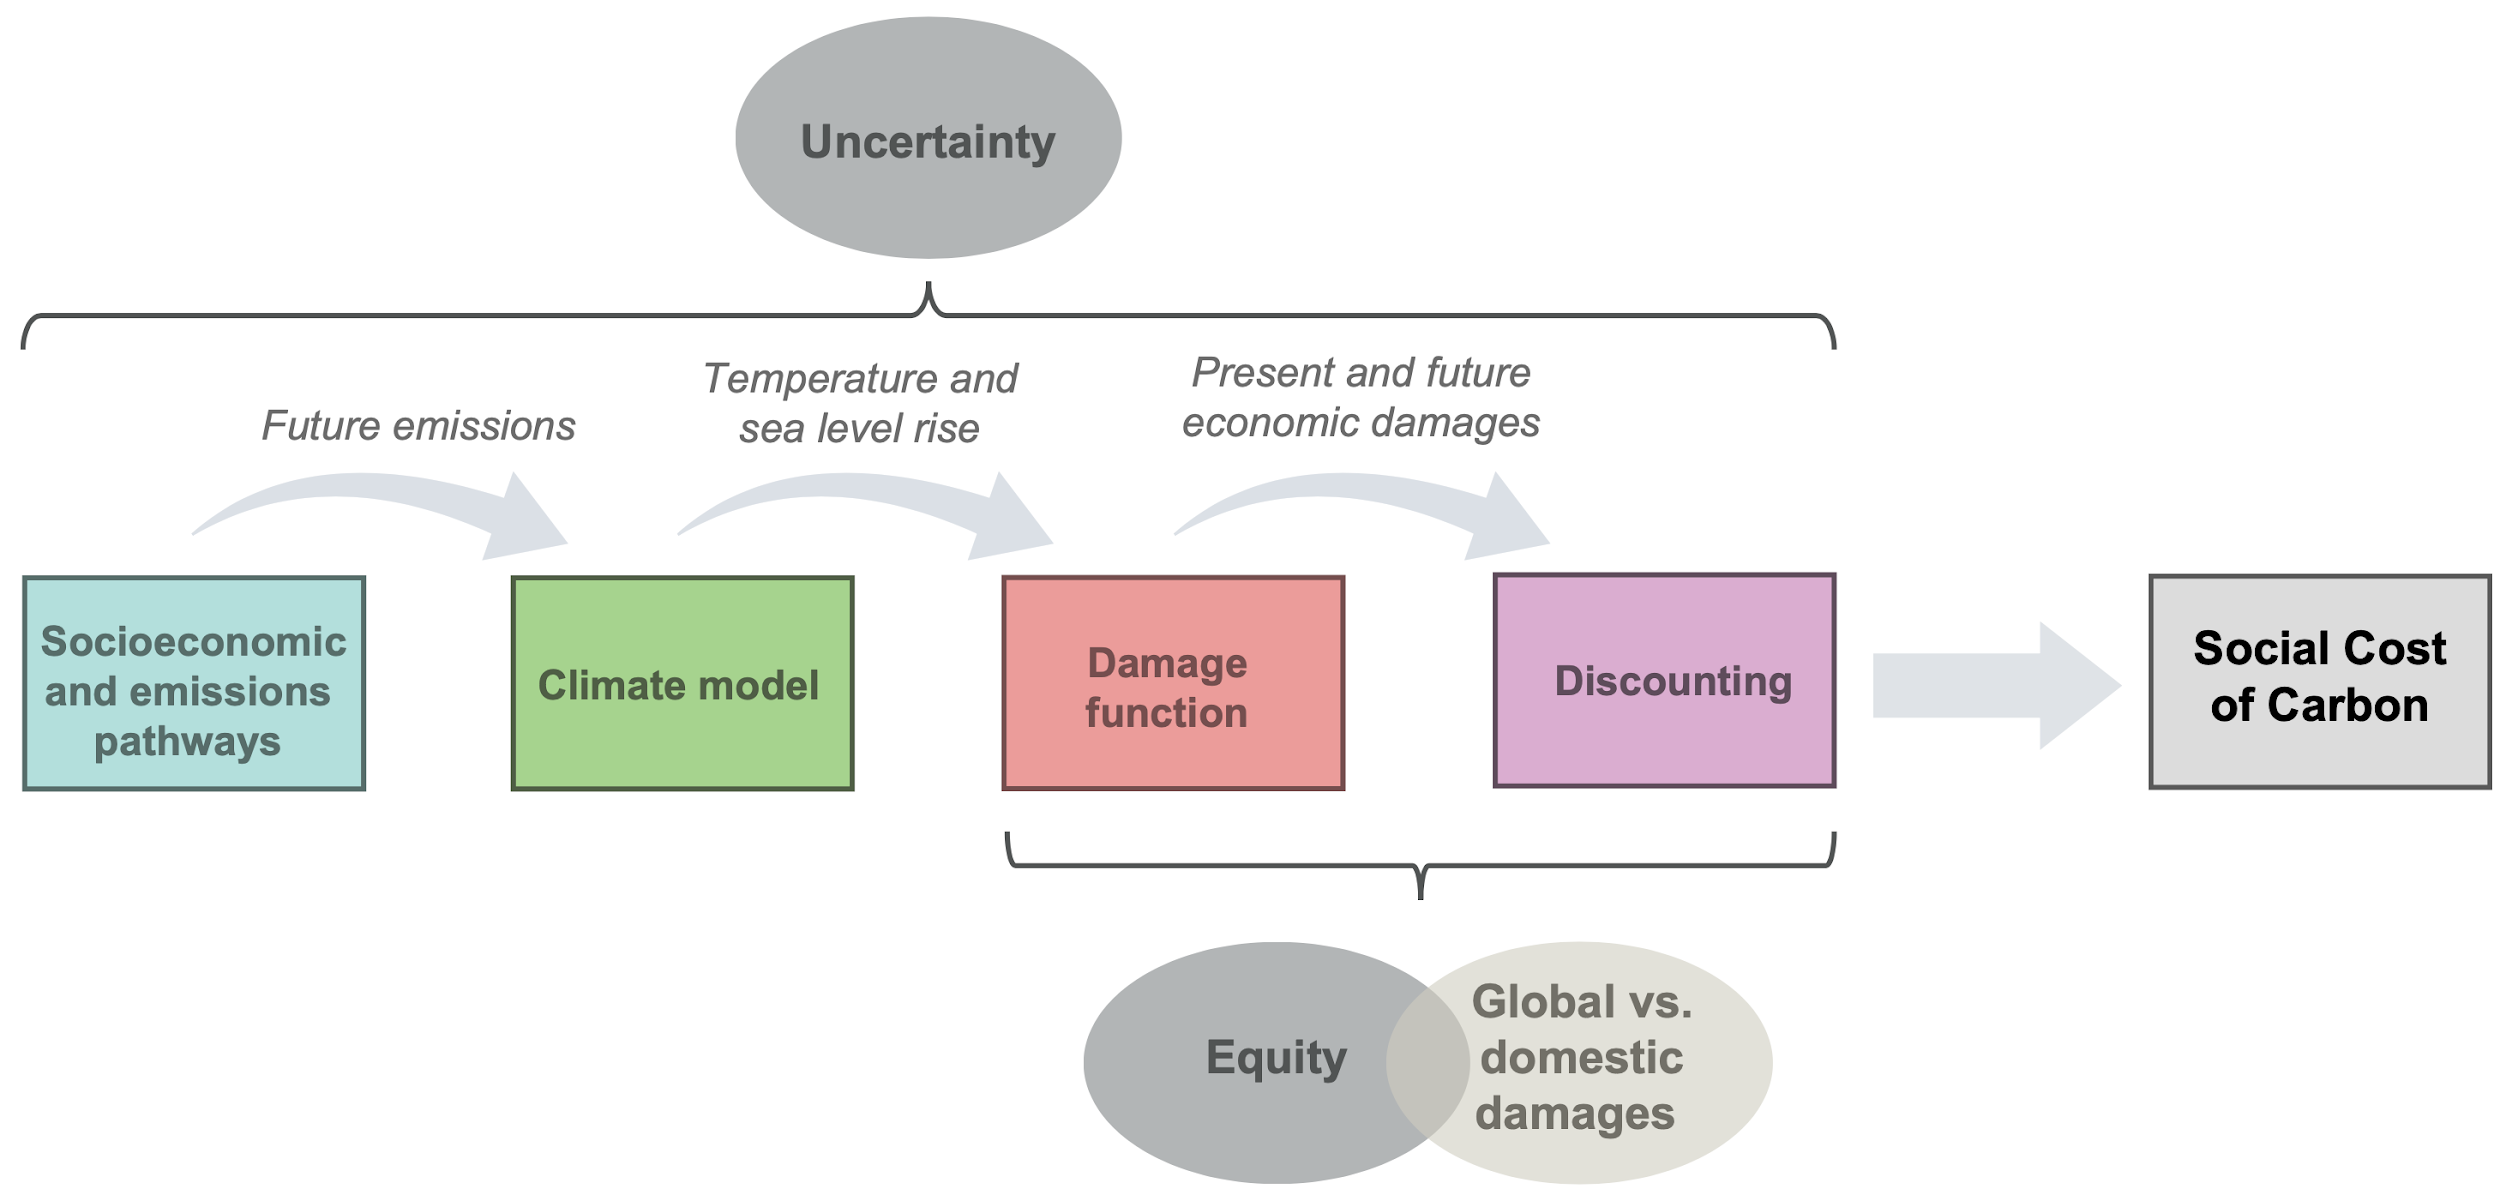
\includegraphics{fig/scc_steps.png}

DICE, FUND, and PAGE substantially
underestimate the speed of temperature increase, relative to climate models that satisfy
the NAS criteria for meeting scientific standards (Figure 4). 17 For example, higher
atmospheric CO 2 concentrations cause the oceans to warm and acidify, which makes
them less effective at removing CO 2 from the atmosphere. The consequence is a positive
feedback loop that accelerates warming. 18 However, this dynamic is missing from both
the DICE and PAGE climate modules.
The delayed projection
of warming in the IAMs' climate models means that resulting estimates of the SCC are
likely to be too low. The delay pushes warming further into the future, which is
discounted more heavily.

A simple Earth system model that can conduct uncertainty analysis while also
matching predictions from these more complex models is necessary. (FAIR)

A key limitation of FAIR and other simple climate models is that they do not represent
the change in global mean sea level rise (GMSL) due to a marginal change in emissions.
However, statistical methods can be used in combination with long historical records of
both temperature and sea level to build a semi-empirical model of the relationship
between GMSL and GMST. 25 Such models are readily available 26 and can enable the
inclusion of marginal damages due both to warming and to projected changes in sea
level. An important potential caveat is that available semi-empirical models of GMSL,
in addition to more complex bottom-up models, may underestimate future sea level rise
due to their inability to capture plausible future dynamics that are not observed in the
historical record (e.g., ice cliff collapse).

At least two problems have plagued the IAM damage functions. First, they are
primarily derived from ad-hoc assumptions and simplified relationships, not large-scale
empirical evidence. Further, the IAM damage functions have tended to treat the world
as nearly homogeneous, dividing the globe into at most sixteen regions. This aggregation
misses a great deal, especially because there are important nonlinearities in the
relationship between temperature and human well-being that are obscured by
substantial aggregation.

The damage functions from FUND, DICE, and PAGE used by the IWG do not
meet this criterion. They are only loosely calibrated to empirical evidence and/or
rely on outdated estimates that fail to isolate the role of changes in the climate
from economic variables such as income and institutions. For example, the
majority of the studies used in FUND's sector-specific damage functions were
published prior to 2000, and all likely suffer from the influence of unobserved
factors that are correlated with temperature. Similarly, early versions of DICE
utilized a damage function that was only loosely tied to empirical literature (Diaz
and Moore, 2017; Nordhaus, 2010), while the recent DICE update continues to
rely on empirical papers that fail to identify plausibly causal effects (Nordhaus
and Moffat, 2017).

Dramatic reductions in computing costs and increased data availability have
enabled researchers to identify the effects of climate change on social and
economic conditions at local scale across the globe. This body of work has
uncovered that many socioeconomic outcomes display a strongly nonlinear
relationship with climate variables.

The existing IAMs' damage functions fail to adequately characterize
nonlinearities, to disaggregate local impacts around the world, or to include
information from lower-income, hotter regions of the globe.

Overturned past findings that suggested that
climate change would benefit agriculture, instead finding that it would cause substantial
damage.

Along with a set of socioeconomic and emissions scenarios, discussed below,
the climate and damages modules together translate a single additional ton of CO2
emissions into a trajectory of additional warming, and a stream of future damages. The
final step in the SCC calculation is to express this stream of damages as a single present
value, so that future costs and benefits can be directly compared to costs and benefits of
actions taken today.

!!
There are two reasons for ``discounting the future,'' or more precisely for discounting
future monetary amounts, whether benefits or costs. The first is that an additional
dollar is worth more to a poor person than a wealthy one, which is referred to in
technical terms as the declining marginal value of consumption. The relevance for the
SCC is that damages from climate change that occur in the future will matter less to
society than those that occur today, because societies will be wealthier. The second,
which is debated more vigorously, is the pure rate of time preference: people value the
future less than the present, regardless of income levels. While individuals may
undervalue the future because of the possibility that they will no longer be alive, it is
unclear how to apply such logic to society as a whole facing centuries of climate change.
Perhaps the most compelling explanation for a nonzero pure rate of time preference is
the possibility of a disaster (e.g., asteroids or nuclear war) that wipes out the population
at some point in the future, thus removing the value of any events that happen
afterwards.

!!
U.S. government agencies have relied on the Office of Management and
Budget's (OMB's) guidance to federal agencies on the development of regulatory
analysis in Circular A-4, and used 3 percent and 7 percent discount rates in cost-benefit
analysis. 61 These two values are justified based on observed market rates of return,
which can be used to infer the discount rate for the SCC since any expenditures
incurred today to mitigate CO 2 emissions must be financed just like any other
investment. The 3 percent discount rate is a proxy for the real, after-tax riskless interest
rate associated with U.S. government bonds and the 7 percent rate is intended to reflect
real equity returns like those in the stock market. However, climate change involves
intergenerational tradeoffs, raising difficult scientific, philosophical and legal questions
regarding equity across long periods of time. There is no scientific consensus about the
correct approach to discounting for the SCC.

The assumption that climate damages were projected to be uncorrelated with overall market
returns (eliminating the 7 percent rate, derived from equity markets) and thus used
insights from asset pricing theory that the riskless interest rate was appropriate.

The equilibrium real interest rate has declined substantially since the 1990s,
suggesting a lower discount rate is justified. 65 Additionally, evidence from long-term real
estate investments suggests that for climate mitigation, which has payoffs over very long
periods of time, discount rates should be even lower than those used to discount costs
and benefits of shorter-lived investments. 66 Overall, our judgement is that it is difficult
to defend a 3 percent discount rate for climate investments and there is now a
compelling case for a riskless discount rate of no higher than 2 percent.

!!
There is also the possibility, however, that the riskless rate itself is not appropriate as
the central discount rate due to the unique risk properties of climate change and
uncertainty about future interest rates. Because discount rates reflect the returns to
investments that mitigate climate change, Americans are best served by using an
interest rate associated with investments that match the structure of payoffs from
climate mitigation. Capital asset pricing models recommend low discount rates in
scenarios where investments (in this case CO 2 mitigation) pay off in ``bad'' states of the
world---that is, if climate damages are likely to coincide with a slowing overall economic
growth rate that for example could be due ``tipping points'' or large-scale human
responses to climate change, including mass migration. 68 If on the other hand climate
damages act as tax on the economy (i.e., total damages are larger when the economy
grows faster), then higher discount rates like the average return in equity markets would
be merited.

\emph{Ramsey}
A second potential approach to deriving a discount rate is to explicitly account for
future economic growth using the so-called Ramsey equation, 69 which is often referred to
as the prescriptive approach. This approach has been recommended by the NAS as a
``feasible and conceptually sound framework''. Rather than rely on observed
interest rates, it derives a discount rate from assumptions about three parameters: the
pure rate of time preference, the growth rate of consumption, and a parameter capturing
the decreasing marginal utility of consumption. Values for the first and third parameters
have been estimated in a large literature, while the consumption growth rate will depend
on the set of socioeconomic scenarios developed in the socioeconomic and emissions
module described above. 70
The Ramsey approach has two key limitations. First, future economic growth is
uncertain, while the Ramsey equation is deterministic. Second, climate damages are
likely to be the highest in possible future scenarios where economic growth is the lowest.
Both facts imply that climate mitigation policies act as a form of insurance for the
future and imply a lower discount rate than is given by the Ramsey equation. Besides
these limitations, some find it unappealing that the Ramsey approach requires several
judgments by ``experts'' about the value of key parameters, rather than relying on
observed market interest rates.

\emph{Socioeconomic and Emissions Module}
To calculate the SCC, it is necessary to compare a baseline trajectory of
economic growth and CO 2 emissions to a trajectory in which one more ton of CO 2 is
released. All else equal, a higher baseline CO 2 emissions trajectory will result in a
greater SCC, because projected climate change damages are nonlinear; that is, an
additional ton of CO 2 emissions is projected to cause more damages at higher
atmospheric concentrations of CO 2 .
Baseline economic growth affects the SCC in a
variety of competing ways. Richer economies consume more energy and generate higher
emissions, such that marginal tons do more damage and populations have higher
willingness-to-pay to avoid climate change, which increases the SCC.

\emph{Uncertainty}
In the last decade, advances in
computing have enabled probabilistic climate change projections that capture multiple
measures of uncertainty about the magnitude of climate damages. Thus, for the first
time, it is possible to characterize these uncertainties and to incorporate them into the
calculation of the SCC.
Accounting for this uncertainty when individuals are modeled as risk averse can
substantially increase the SCC.

\emph{Equity}
An additional dollar is worth more to a poor person than a wealthy one.
Applying this principle to the SCC would require ``equity weighting''.
This logic would mean
that damages occurring in poor countries are weighted more highly than damages in
wealthy countries.
The same logic that justifies discounting and the valuation of uncertainty over
future states of the world implies that equity weights should be applied in any SCC
calculation; declining marginal value of consumption is the fundamental economic
concept behind all three concerns. Therefore, the most intellectually coherent approach
to treating equity would be to calibrate equity weights from the large literature studying
the marginal value of consumption, and to apply these weights at the spatial resolution
of damages.

This pathway (C) is based on the recognition that a simple economic principle---declining
marginal value of consumption---underlies the motivation for discounting as well as the
valuation of both equity and uncertainty. 100 This principle is based on the
straightforward observation that \$100 is worth more to a person living in poverty than a
wealthy person. In the climate setting, declining marginal value implies that one should
attach a higher value to future and present impacts of climate change when they occur
to populations experiencing lower incomes. It also means that when future incomes are
uncertain, one has to account for the risk of severe damages occurring when average
global income is very low, and thus when the value of an additional dollar is relatively
high.

Therefore, an argument can be made for computing an SCC in which the damage
function represents the difference in the ``certainty-equivalent'' value of consumption
across all years, populations, and possible future states of the world with and without
climate change. 102 In this approach, the valuation of climate damages is conducted from
the perspective of a person who does not know their circumstances in advance, so they
account for all potential income levels and degrees of climate risk they might face.

Under this approach, discounting, uncertainty valuation, and accounting for equity
implications are all incorporated into the construction of a single, certainty-equivalent
damage function.

\href{Greenstone_2021_Updating_SCC.pdf}{Carleton Greenstone (2021) Updating SCC (pdf)}

\href{http://www.impactlab.org/}{Climate Impact Lab}

\href{https://fair.readthedocs.io/en/latest/}{FAIR}

\hypertarget{current-prices-far-below-scc}{%
\section{Current Prices far below SCC}\label{current-prices-far-below-scc}}

The vast majority of carbon prices are
well below even the most conservative estimates of the ``social cost of carbon'' (SCC).
The SCC internalizes the environmental and health effects of greenhouse gas emissions. A recent study
surveyed environmental experts on their estimation of SCC, which ranged between \$80 and
\$300 per ton (Pindyck, 2019). Another study estimates a global median price of \$417, with
substantial national level variation (Ricke et al., 2018) A more conservative estimate puts the
SCC between \$50-\$100 by 2030 (Carbon Pricing Leadership Commission, 2017).
Even compared to the most conservative estimates of the SCC, carbon pricing falls short. The
most recent World Bank survey of carbon pricing shows that half of the 61 carbon pricing
policies around the globe have a price lower than \$10. The IMF estimates that the average
global price for carbon is \$2/ton (Parry, 2019).

\href{https://iopscience.iop.org/article/10.1088/1748-9326/abdae9/meta}{Green(2021) Carbon Pricing Ex-Post}
\href{pdf/Green_2021_Carbon_Pricing_Ex-Post.pdf}{(pdf)}

\hypertarget{part-impacts}{%
\part{Impacts}\label{part-impacts}}

\hypertarget{impacts}{%
\chapter{Impacts}\label{impacts}}

Overview of Nature Communications on Climate Change Impacts:

\href{https://www.nature.com/collections/hcfhgcahdc}{Nature Communications}

\hypertarget{water-availability}{%
\section{Water availability}\label{water-availability}}

\emph{Abstract Konapala}

Accessibility of water resources for human consumption and ecosystems largely depends on the spatio-temporal distribution of both precipitation and evaporation.
As a result, changes in characteristics of precipitation and evaporation due to human-caused climate change in the 21st century may result in changes in water availability (WA) that have implications for both humans and the biosphere.
Previous studies have elucidated trends in precipitation in terms of both annual mean, seasonal variation, and the distribution of extreme events. Studies have also examined the corresponding changes in evaporation characteristics.
Though the combined monthly distribution of precipitation and evaporation have widespread implications for regional hydrology, crop yield, and ecology, few studies have examined the concomitant changes in both annual mean and seasonal variation in these variables.
Moreover, the existing global climate classifications that form the basis for WA studies rarely consider seasonal variation characteristics from a non-parametric standpoint, even though they vary in a complex manner across global land regions.

\href{https://www.nature.com/articles/s41467-020-16757-w}{Konapala (2021) Water Availability}
\href{pdf/Konapala_2021_Water_Availability.pdf}{(pdf)}

\hypertarget{part-actions}{%
\part{Actions}\label{part-actions}}

\hypertarget{legal-action}{%
\chapter{Legal Action}\label{legal-action}}

\href{https://youth4climatejustice.org/the-case/}{youth4climate The Case}

\hypertarget{outreach}{%
\chapter{Outreach}\label{outreach}}

Fossil fuel emissions from human activity are driving up Earth's temperature---
yet something else is at work.
The warming has set in motion nature's own feedback loops
which are raising temperatures even higher.
The urgent question is:
Are we approaching a point of no return, leading to an uninhabitable Earth,
or do we have the vision and will to slow, halt, and reverse them?

\href{https://feedbackloopsclimate.com/introduction/}{Feedbackloops 5 Videos}

\hypertarget{part-appendices}{%
\part{Appendices}\label{part-appendices}}

\hypertarget{appendix-appendices}{%
\appendix}


\hypertarget{about}{%
\chapter{About}\label{about}}


\includegraphics{fig/me.jpg}

\emph{Dyre Haugen} and \emph{Dyrehaugen} is Webian for \emph{Jon Martin} -
self-owned Globian, Webian, Norwegian and Canarian with
a background from industrial research policy, urban planning and
economic development consulting on global, regional and urban scales.
I am deeply concerned about the (insane) way
humanity (i.e.~capitalism) interfere with nature.
In an effort to gain insights in how and why this happens
stuff is collected from around the web and put together
in a linked set of web-sites.
The sites are operated as personal notebooks.
However, these days things can be easily published to the
benefit of others concerned with the same issues.
But be aware - this is not polished for presentation or
peer-reviewed for exactness.
I offer you just to have a look at my `work-desk' as it appears in the moment.
Any comment or suggestion can be mailed to \href{mailto:dyrehaugen@gmail.com}{\nolinkurl{dyrehaugen@gmail.com}}
You can follow me on twitter as @dyrehaugen.
Thanks for visiting!

\hypertarget{news}{%
\chapter{NEWS}\label{news}}

\hypertarget{adaptation-summit}{%
\section{210130 Adaptation Summit}\label{adaptation-summit}}

Climate change adaptation seems to be a fairly new concept to many leaders. It were sometimes mix-ups with mitigation during the high-level talks.
Mitigation and adaptation are both important and sometimes they overlap, so mix-ups are understandable.
Climate adaptation involves many communities and disciplines (e.g.~weather forecasting, climate services, regional climate modelling, ``distillation``, disaster risk reduction).

Financing is clearly needed for climate change adaptation. To ensure progress and avoid lofty visions without results on the ground, there may also be a need for tangible results and to show examples and demonstrations. One specific type discussed at the summit was ``Early warning systems'' which play an important role.

But early warning systems, the way I understand them, don't provide information about climate risks on longer timescales. Weather and climate -- short and long timescales -- are of course connected but nevertheless different

\href{http://www.realclimate.org/index.php/archives/2021/01/climate-adaptation-summit-2021/}{Rasmus (2021) Adaptation Summit}

\hypertarget{warming-all-anthropogenic}{%
\section{210118 Warming all anthropogenic}\label{warming-all-anthropogenic}}

Parties to the Paris Agreement agreed to holding global average temperature increases ``well below 2 °C above pre-industrial levels and pursuing efforts to limit the temperature increase to 1.5 °C above pre-industrial levels''. Monitoring the contributions of human-induced climate forcings to warming so far is key to understanding progress towards these goals. Here we use climate model simulations from the Detection and Attribution Model Intercomparison Project, as well as regularized optimal fingerprinting, to show that \emph{anthropogenic forcings caused 0.9 to 1.3 °C of warming in global mean near-surface air temperature in 2010--2019 relative to 1850--1900, compared with an observed warming of 1.1 °C}. Greenhouse gases and aerosols contributed changes of 1.2 to 1.9 °C and −0.7 to −0.1 °C, respectively, and \emph{natural forcings contributed negligibly}. These results demonstrate the substantial human influence on climate so far and the urgency of action needed to meet the Paris Agreement goals.

\href{https://www.nature.com/articles/s41558-020-00965-9}{Nature (paywall)}

\hypertarget{globale-temperature-1880-2020}{%
\section{21014 Globale Temperature 1880-2020}\label{globale-temperature-1880-2020}}

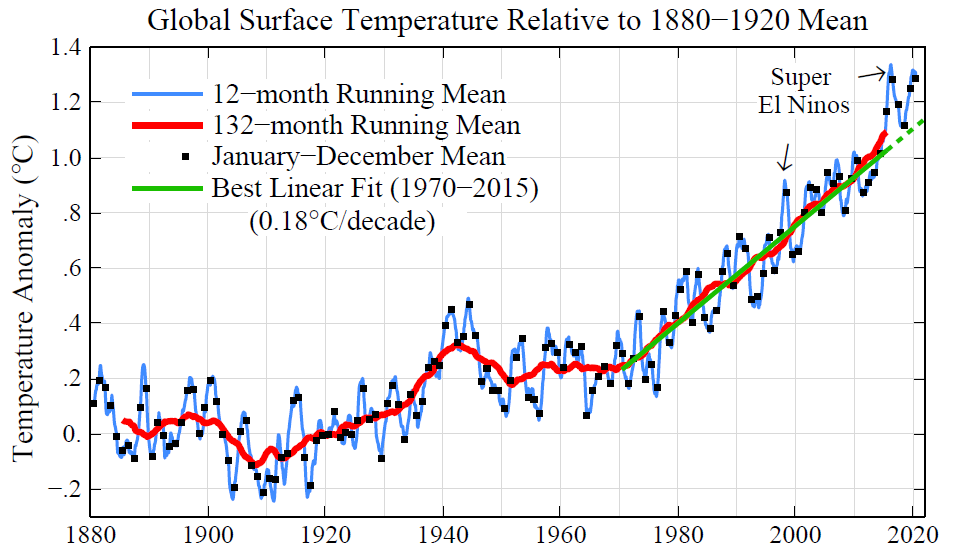
\includegraphics{fig/Global_Temperature_1880-2020.png}

The rate of global warming has accelerated in the past several years. The 2020 global temperature was +1.3°C (\textasciitilde2.3°F) warmer than in the 1880-1920 base period; global temperature in that base period is a reasonable estimate of `pre-industrial' temperature. The six warmest years in the GISS record all occur in the past six years, and the 10 warmest years are all in the 21st century. Growth rates of the greenhouse gases driving global warming are increasing, not declining.

{[}GISSTEMP 2020 Update{]} (\url{https://mailchi.mp/caa/global-temperature-in-2020?e=96d59a909f})

\hypertarget{not-so-long-lag}{%
\section{210104 Not so long lag?}\label{not-so-long-lag}}

\begin{quote}
Until recently, Mann explained in The Guardian, scientists believed the climate system---a catch-all term for the interaction among the Earth's atmosphere, oceans, and other parts of the biosphere---carried a long lag effect. This lag effect was mainly a function of carbon dioxide remaining in the atmosphere and trapping heat for many decades after being emitted. So, even if humanity halted all CO2 emissions overnight, average global temperatures would continue to rise for 25 to 30 years, while also driving more intense heat waves, droughts, and other climate impacts. Halting emissions will take at least twenty years, under the best of circumstances, and so humanity was likely locked in to at least 50 more years of rising temperatures and impacts.
\end{quote}

\begin{quote}
Research over the past ten years, however, has revised this vision of the climate system. Scientists used to ``treat carbon dioxide in the atmosphere as if it was a simple control knob that you turn up'' and temperatures climb accordingly, ``but in the real world we now know that's not what happens,'' Mann said. Instead, if humans ``stop emitting carbon right now \ldots{} the oceans start to take up carbon more rapidly.'' The actual lag effect between halting CO2 emissions and halting temperature rise, then, is not 25 to 30 years but, per Mann, ``more like three to five years.''
(October 2020)
\end{quote}

\href{https://www.theguardian.com/us-news/2020/oct/02/donald-trump-climate-change-michael-mann-interview}{Guardian article}

\href{https://www.cjr.org/covering_climate_now/michael-mann-60-minutes-emissions-warming.php}{Covering Climate Now article}

\hypertarget{climate-finance-shadow-report-2020}{%
\section{210102 Climate Finance Shadow Report 2020}\label{climate-finance-shadow-report-2020}}

Oxfam has released this report with subtitle \emph{Asessing progress towards the \$100 billion commitment}
Progress is NOT in line with need or pledges.

\begin{quote}
Climate change could undo decades of progress in development and dramatically increase global inequalities. There is an urgent need for climate finance to help countries cope and adapt.
Over a decade ago, developed countries committed to mobilize \$100bn per year by 2020 to support developing countries to adapt and reduce their emissions. The goal is a critical part of the Paris Agreement.
As 2020 draws to a close, Oxfam's Climate Finance Shadow Report 2020 offers an assessment of progress towards the \$100bn goal.
\end{quote}

\begin{quote}
Based on 2017--18 reported numbers, developed countries are likely to claim they are on track to meet
the \$100bn goal. And on their own terms, they may be. But how the goal is met is as important as whether
it is met. The dubious veracity of reported numbers, the extent to which climate finance is increasing
developing country indebtedness, and the enduring gap in support for adaptation, LDCs and SIDS, are grave
concerns. Meeting the \$100bn goal on these terms would be cause for concern, not celebration.
\end{quote}

\href{https://www.oxfam.org/en/research/climate-finance-shadow-report-2020}{Oxfam Report}
\href{/pdf/Oxfam_2020_Climate_Finance_Shadow_Report.pdf}{(pdf)}

  \bibliography{book.bib,packages.bib}

\end{document}
